%\setcounter{chapter}{9}
\chapter{Gradient-Based Learning Algorithms}\label{chapter-gradient_descent}


\section{Introduction}

Once you have specified a learning problem (loss function, hypothesis space, parameterization), the next step is to find the parameters that minimize the loss. This is an optimization problem, and the most common optimization algorithm we will use is \index{Gradient descent}\textbf{gradient descent}. Gradient descent is like a skier making their way down a snowy mountain, where the shape of the mountain is the loss function.

There are many varieties of gradient descent, and we will call this whole family \textbf{gradient-based learning algorithms}. All share the same basic idea: at some operating point, calculate the direction of steepest descent, then use this direction to find a new operating point with lower loss.\marginnote{We use the term \textbf{operating point} to refer to a particular point (setting of the parameters) where we are currently evaluating the loss.}[-0.85cm]

\section{Technical Setting}
In this chapter, we consider the task of minimizing a cost function $J: \cdot \rightarrow \mathbb{R}$, which is a function that maps some arbitrary input to a scalar cost. %The domain of this function can be anything, but the range is always a scalar.

In learning problems, the domain of $J$ is the training data and the parameters $\theta$.\marginnote{Remember from \chap{\ref{chapter-intro_to_learning}} that in supervised learning, the training data is $\{\mathbf{x}^{(i)}, \mathbf{y}^{(i)}\}^N_{i=1}$, while in unsupervised learning the training data is $\{\mathbf{x}^{(i)}\}^N_{i=1}$.} Often, we will consider the training data to be fixed and only denote the objective as a function of the parameters, $J(\theta)$. Our goal is to solve:
\begin{align}
    \theta^* = \argmin_{\theta} J(\theta)
\end{align}

%When we evaluate $J$ at some specific location $\theta$, we will say that is the value of $J$ at operating point $\theta$. 

%$\nabla_{\theta} J \triangleq \frac{\partial J}{\partial \theta}$

Pretty much all optimizers work by some iterative process, where they update the parameters to be better and better. Different optimizers differ in how the parameter update function works. The update function gets to view some information about the loss landscape, then uses that information to update the parameters, as shown in \fig{\ref{fig-gradient_descent-optimization_schematic}}.
\begin{figure}[h]
    \centerline{
    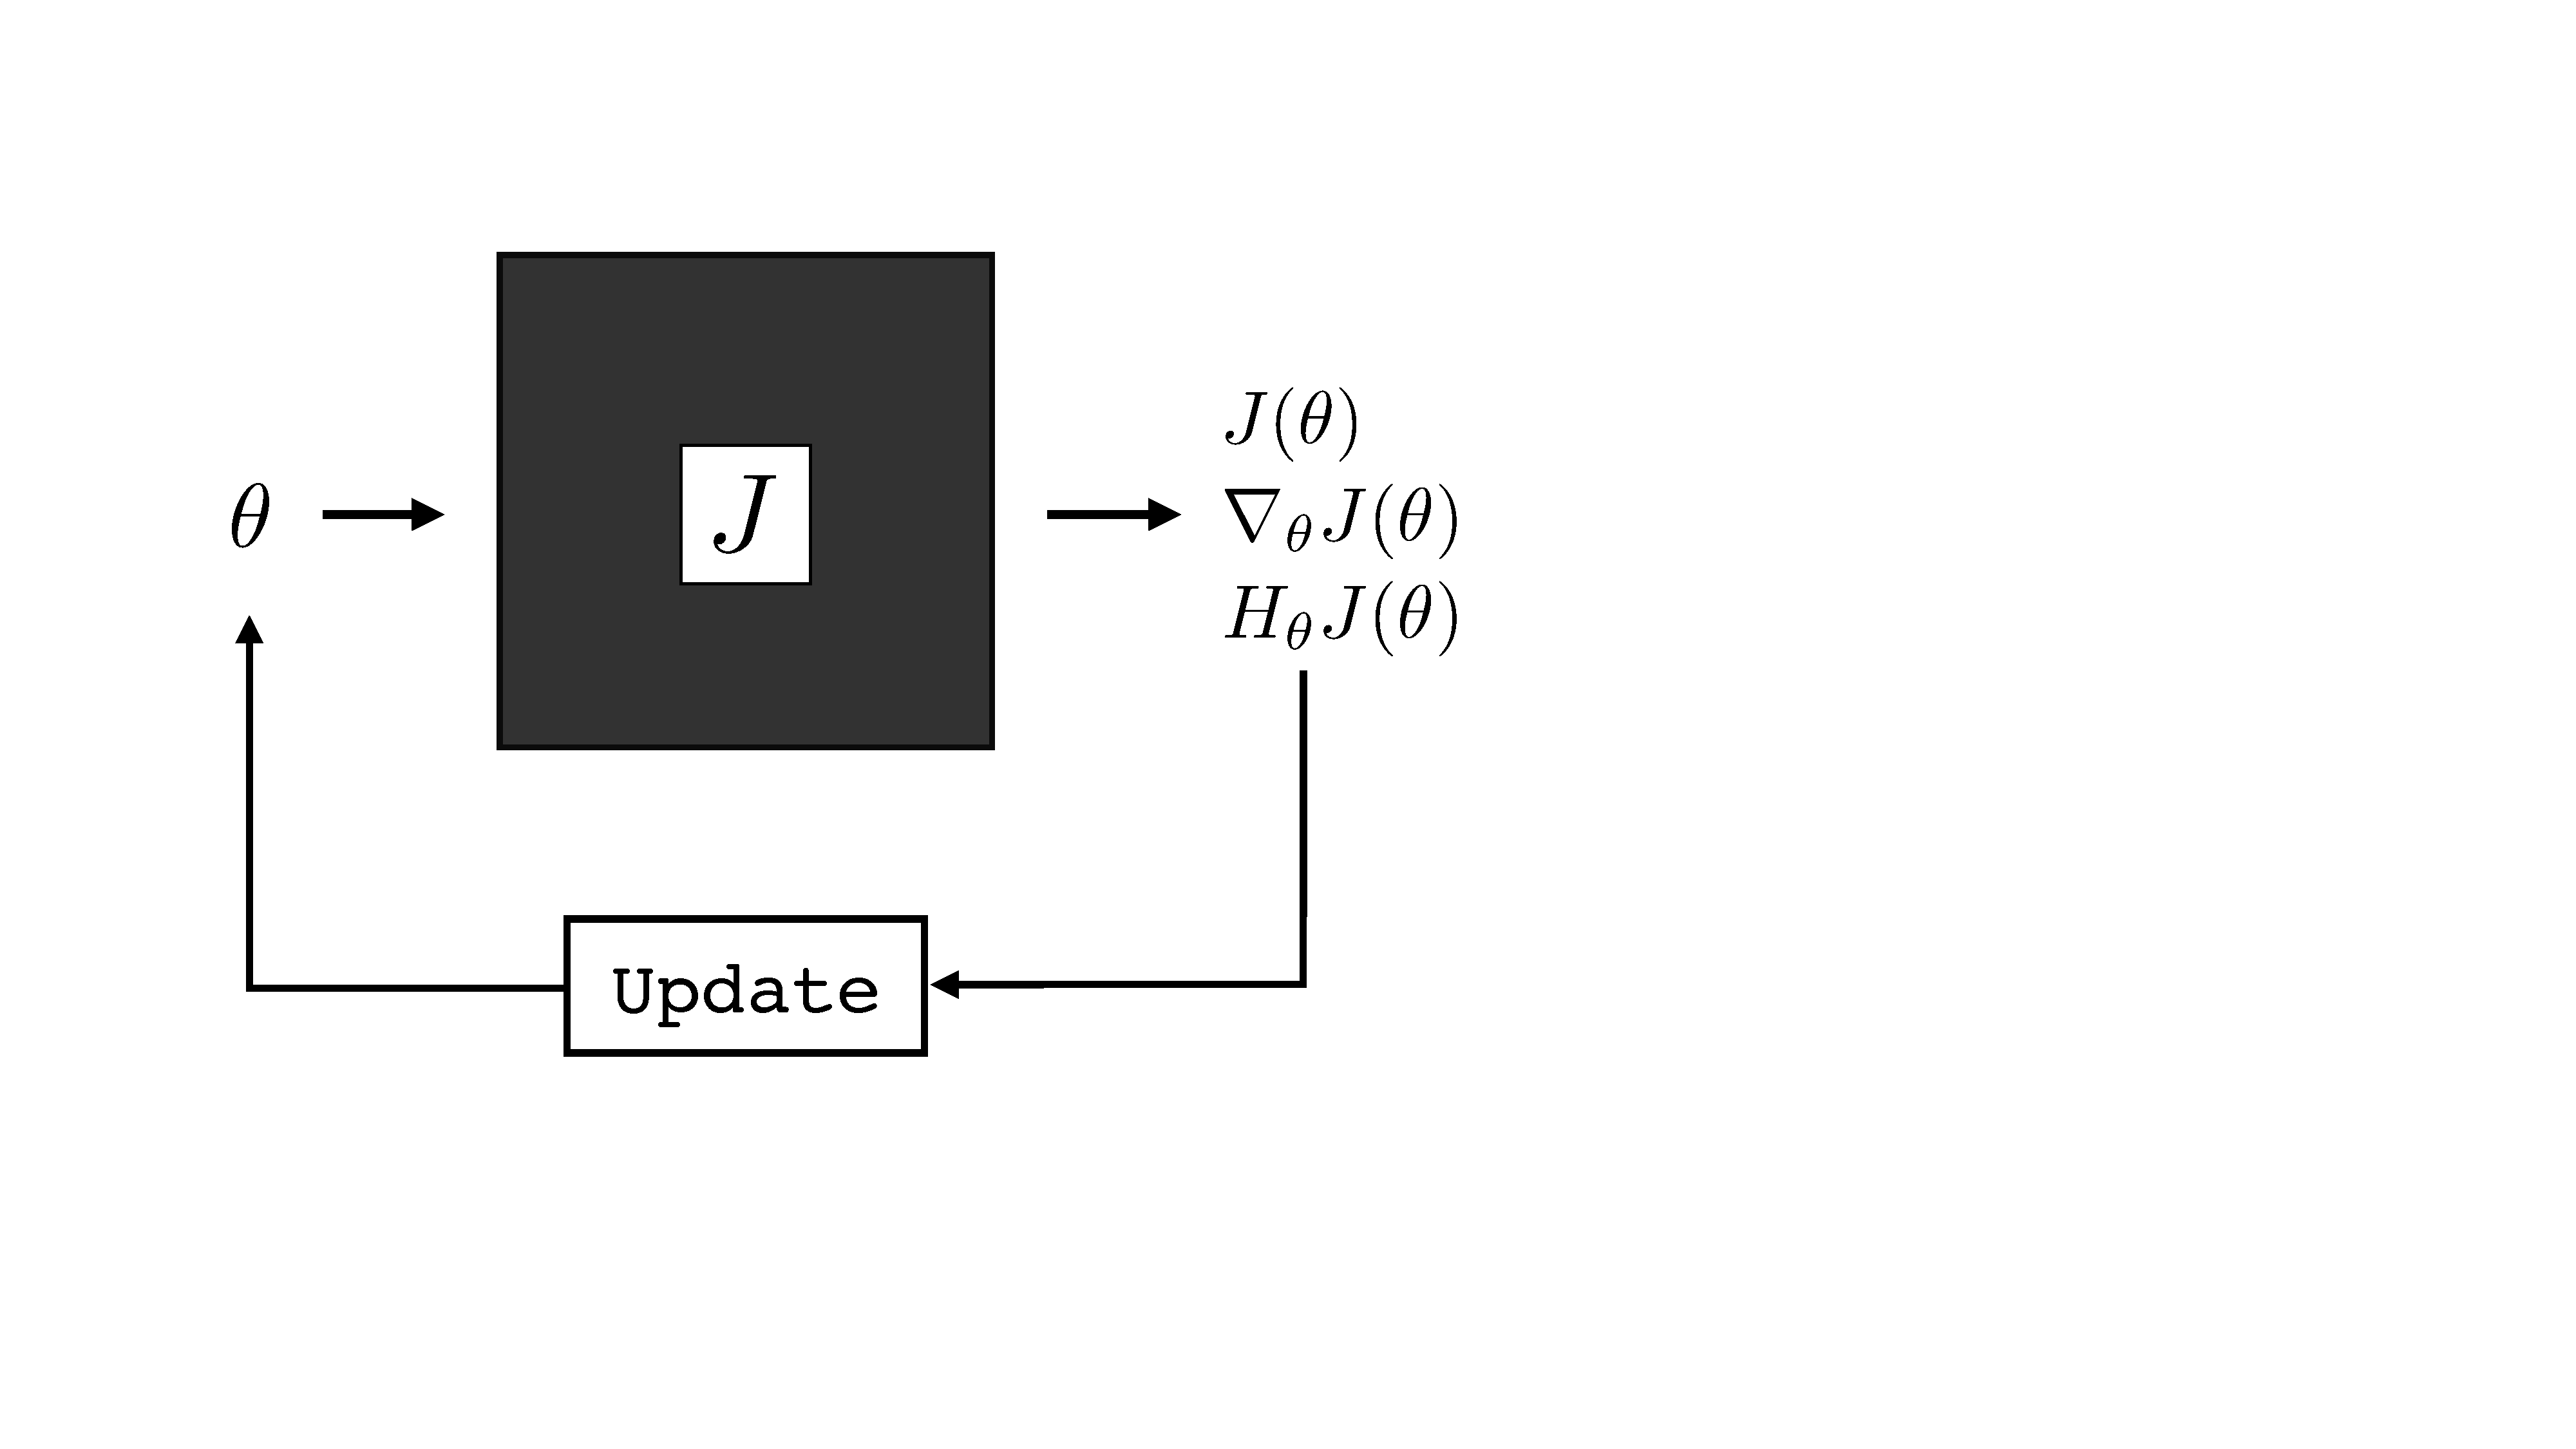
\includegraphics[width=0.35\linewidth]{./figures/gradient_descent/optimization_schematic.pdf}
    }
    \caption{General optimization loop.}
    \label{fig-gradient_descent-optimization_schematic}
\end{figure}

In the simplest setting, called \index{Zeroth-order optimization}\textbf{zeroth-order optimization}, the update function only gets to observe the value $J(\theta)$. The only way, then, to find $\theta$'s that minimize the loss is to sample different values for $\theta$ and move toward the values that are lower.

For gradient-based optimization, also called \index{First-order optimization}\textbf{first-order optimization}, the update function takes as input the gradient of the cost with respect to the parameters at the current operating point, $\nabla_{\theta}J(\theta)$. This reveals hugely useful information about the loss that directly tells us how to minimize it: just move in the direction of steepest descent, that is, the gradient direction.

Higher-order optimization methods observe higher-order derivatives of the loss, such as the Hessian $H$, which tells you how the landscape is locally curving. The Hessian is costly to compute but many methods use approximations to the Hessian, or other properties related to loss curvature, and these are growing in popularity~\cite{martens2015optimizing,foret2020sharpness}.


\section{Basic Gradient Descent}
The simplest version of gradient descent just takes a step in the gradient direction of length proportional to the gradient magnitude. This algorithm is described in \algref{\ref{alg-gradient_descent-basic_gradient_descent}}.
\begin{algorithm}[h]
\SetAlgoVlined
\DontPrintSemicolon
%\marginnote{{\bf Algorithm \ref{alg-gradient_descent-basic_gradient_descent}}: Optimizing a cost function $J: \theta \rightarrow \mathbb{R}$ by descending the gradient $\nabla_{\theta} J$.}
\caption{{\bf Algorithm \ref{alg-gradient_descent-basic_gradient_descent}}: Gradient descent (\texttt{GD}). Optimizing a cost function $J: \theta \rightarrow \mathbb{R}$ by descending the gradient $\nabla_{\theta} J$.}
\fakealgorithmcaption{}
\label{alg-gradient_descent-basic_gradient_descent}
{\bf Input:} objective function $J$, initial parameter vector $\theta^0$, learning rate $\eta$, number of steps $K$\;%, data $\{\mathbf{x}^{(i)},\mathbf{y}^{(i)}\}_{i=1}^N$
{\bf Output:} trained parameter vector $\theta^* = \theta^K$\;
\For{\upshape $k= 0, \dots, K-1$}{
    %$J = \sum_{i=1}^N \mathcal{L}(f_{\theta^{k}}(\mathbf{x}^{(i)}),\mathbf{y}^{(i)})$\;
    $\theta^{k+1} \leftarrow \theta^{k} - \eta \nabla_{\theta} J(\theta^k)$\;
}
\end{algorithm}

This algorithm has two hyperparameters, the \index{Learning rate}\textbf{learning rate} $\eta$, which controls the step size (learning rate times gradient magnitude), and the number of steps $K$. If the learning rate is sufficiently small and the initial parameter vector $\theta^0$ is random, then this algorithm will almost surely converge to a local minimum of $J$ as $K \rightarrow \infty$~\cite{lee2016gradient}. However, to descend more quickly, it can be useful to set the learning rate to a higher value. 

\section{Learning Rate Schedules}
A generally useful strategy is to start with a high value for $\eta$ and then decay it until convergence according to a \textbf{learning rate schedule}. Researchers have come up with innumerable schedules and they generally work by calling some function $\texttt{lr}(\eta^0,k)$ to get the learning rate on each iteration of descent:
\begin{align}
    \eta^{k} = \texttt{lr}(\eta^0,k)
\end{align}
Generally, we want an update rule where $\eta^{k+1} < \eta^k$, so that we take smaller steps as we approach the minimizer. A few simple and popular approaches are given below:
\begin{align}
    \texttt{lr}(\eta^0,k) &= \beta^{-k} \eta^0 &\quad\quad \triangleleft\quad \text{exponential decay}\\
    \texttt{lr}(\eta^0,k) &= \beta^{-\lfloor k/M \rfloor} \eta^0 &\quad\quad \triangleleft\quad \text{stepwise exponential decay}\\
    \texttt{lr}(\eta^0,k) &= \frac{(K - k)}{K} \eta^0 &\quad\quad \triangleleft\quad \text{linear decay}
\end{align}
\marginnote{One downside of linear decay is that it depends on the total number of steps $K$. This makes it hard to compare optimization runs of different lengths. This is something to also be aware of in more advanced learning rate schedules, such as cosine decay~\cite{loshchilov2016sgdr}, which also have different behavior for different settings of $K$.}[-3.2cm]
The $\beta$ and $M$ are additional hyperparameters of these methods. The general approach of learning rate decay is summarized in \algref{\ref{alg-gradient_descent-gradient_descent_with_lr_decay}}.

%but a simple one that tends to work decently is to just multiply the $\eta$ by a  constant factor $\beta \in (0,1)$ every iteration of gradient descent, where $\beta$ and the initial learning rate $\eta^1$ are the new hyperparameters to specify. 
\begin{algorithm}[h]
\SetAlgoVlined
\DontPrintSemicolon
%\marginnote{{\bf Algorithm \ref{alg-gradient_descent-gradient_descent_with_lr_decay}}: Gradient descent with a learning rate schedule.}
\caption{{\bf Algorithm \ref{alg-gradient_descent-gradient_descent_with_lr_decay}}: Gradient descent with a learning rate schedule.}
%\caption{{\bf Algorithm \ref{alg-gradient_descent-gradient_descent_with_lr_decay}}: \texttt{GD}+\texttt{lr}-schedule.}
\fakealgorithmcaption{}
\label{alg-gradient_descent-gradient_descent_with_lr_decay}
{\bf Input:} objective function $J$, initial parameter vector $\theta^0$, initial learning rate $\eta^0$, learning rate function $\texttt{lr}$, number of steps $K$\;%, data $\{\mathbf{x}^{(i)},\mathbf{y}^{(i)}\}_{i=1}^N$
{\bf Output:} trained parameter vector $\theta^* = \theta^K$\;
\For{\upshape $k= 0, \dots, K-1$}{
    %$J = \sum_{i=1}^N \mathcal{L}(f_{\theta^{k-1}}(\mathbf{x}^{(i)}),\mathbf{y}^{(i)})$\;
    $\eta^{k} \leftarrow \texttt{lr}(\eta^0, k)$\;
    $\theta^{k+1} \leftarrow \theta^{k} - \eta^{k} \nabla_{\theta} J(\theta^k)$\;
}
\end{algorithm}

Variations on this algorithm include only decaying the learning rate when a plateau is reached (i.e., when the loss is not decreasing for many iterations in a row), or decaying the learning rate according to more complex nonlinear schedules, such as one shaped like a cosine function~\cite{loshchilov2016sgdr}.%once every $M$ steps of gradient descent, for some fixed value $M$ (which becomes an additional hyperparameter of the algorithm).

\section{Momentum}
Could we do a smarter update than just taking a step in the direction of the gradient? Of the countless ideas that have been proposed, one of the few that has stuck is \index{Momentum}\textbf{momentum}~\cite{polyak1964some,sutskever2013importance}. Momentum makes the analogy to skiing even more precise: momentum is like the inertia of the skier, carrying them over the little bumps and imperfections in the ski slope and increasing their speed as they descend along a straight path. In math, momentum just means that we set the parameter update to be a direction $\mathbf{v}^{k+1}$, given by a weighted combination of the previous update direction, $\mathbf{v}^{k}$, plus the current negative gradient:
\begin{align}
    \mathbf{v}^{k+1} = \mu \mathbf{v}^{k} - \eta\nabla_{\theta} J(\theta^k)
\end{align}
The weight $\mu$ in this combination is a new hyperparameter, sometimes simply called the momentum. The full algorithm is given in \algref{\ref{alg-gradient_descent-gradient_descent_with_momentum}}.
\begin{algorithm}[h]
\SetAlgoVlined
\DontPrintSemicolon
%\marginnote{{\bf Algorithm \ref{alg-gradient_descent-gradient_descent_with_momentum}}: Gradient descent with momentum.}
\caption{{\bf Algorithm \ref{alg-gradient_descent-gradient_descent_with_momentum}}: Gradient descent with momentum.}
\fakealgorithmcaption{}
\label{alg-gradient_descent-gradient_descent_with_momentum}
{\bf Input:} objective function $J$, initial parameter vector $\theta^0$, learning rate $\eta$, momentum $\mu$, number of steps $K$\;%, data $\{\mathbf{x}^{(i)},\mathbf{y}^{(i)}\}_{i=1}^N$
{\bf Output:} trained parameter vector $\theta^* = \theta^K$\;
$\mathbf{v}^{0} = \mathbf{0}$\;
\For{\upshape $k= 0, \dots, K-1$}{
    $\mathbf{v}^{k+1} = \mu \mathbf{v}^{k} - \eta\nabla_{\theta} J(\theta^k)$\;
    $\theta^{k+1} \leftarrow \theta^{k} + \mathbf{v}^{k+1}$\;
}
\end{algorithm}

\Fig{\ref{fig-gradient_descent-momentum_out1}} shows how momentum affects gradient descent for a simple objective $J = \texttt{abs}(\theta)$ (absolute value of $\theta$). As can be seen in the figure, some momentum can help convergence rate (\fig{\ref{fig-gradient_descent-momentum_out1}}, $\mu = 0.5$) but too much momentum will cause the trajectory to overshoot the optimum and even when the optimum loss is achieved, the trajectory might not stop (\fig{\ref{fig-gradient_descent-momentum_out1}}, $\mu = 0.95$).

\begin{figure}[h]
    \centering
    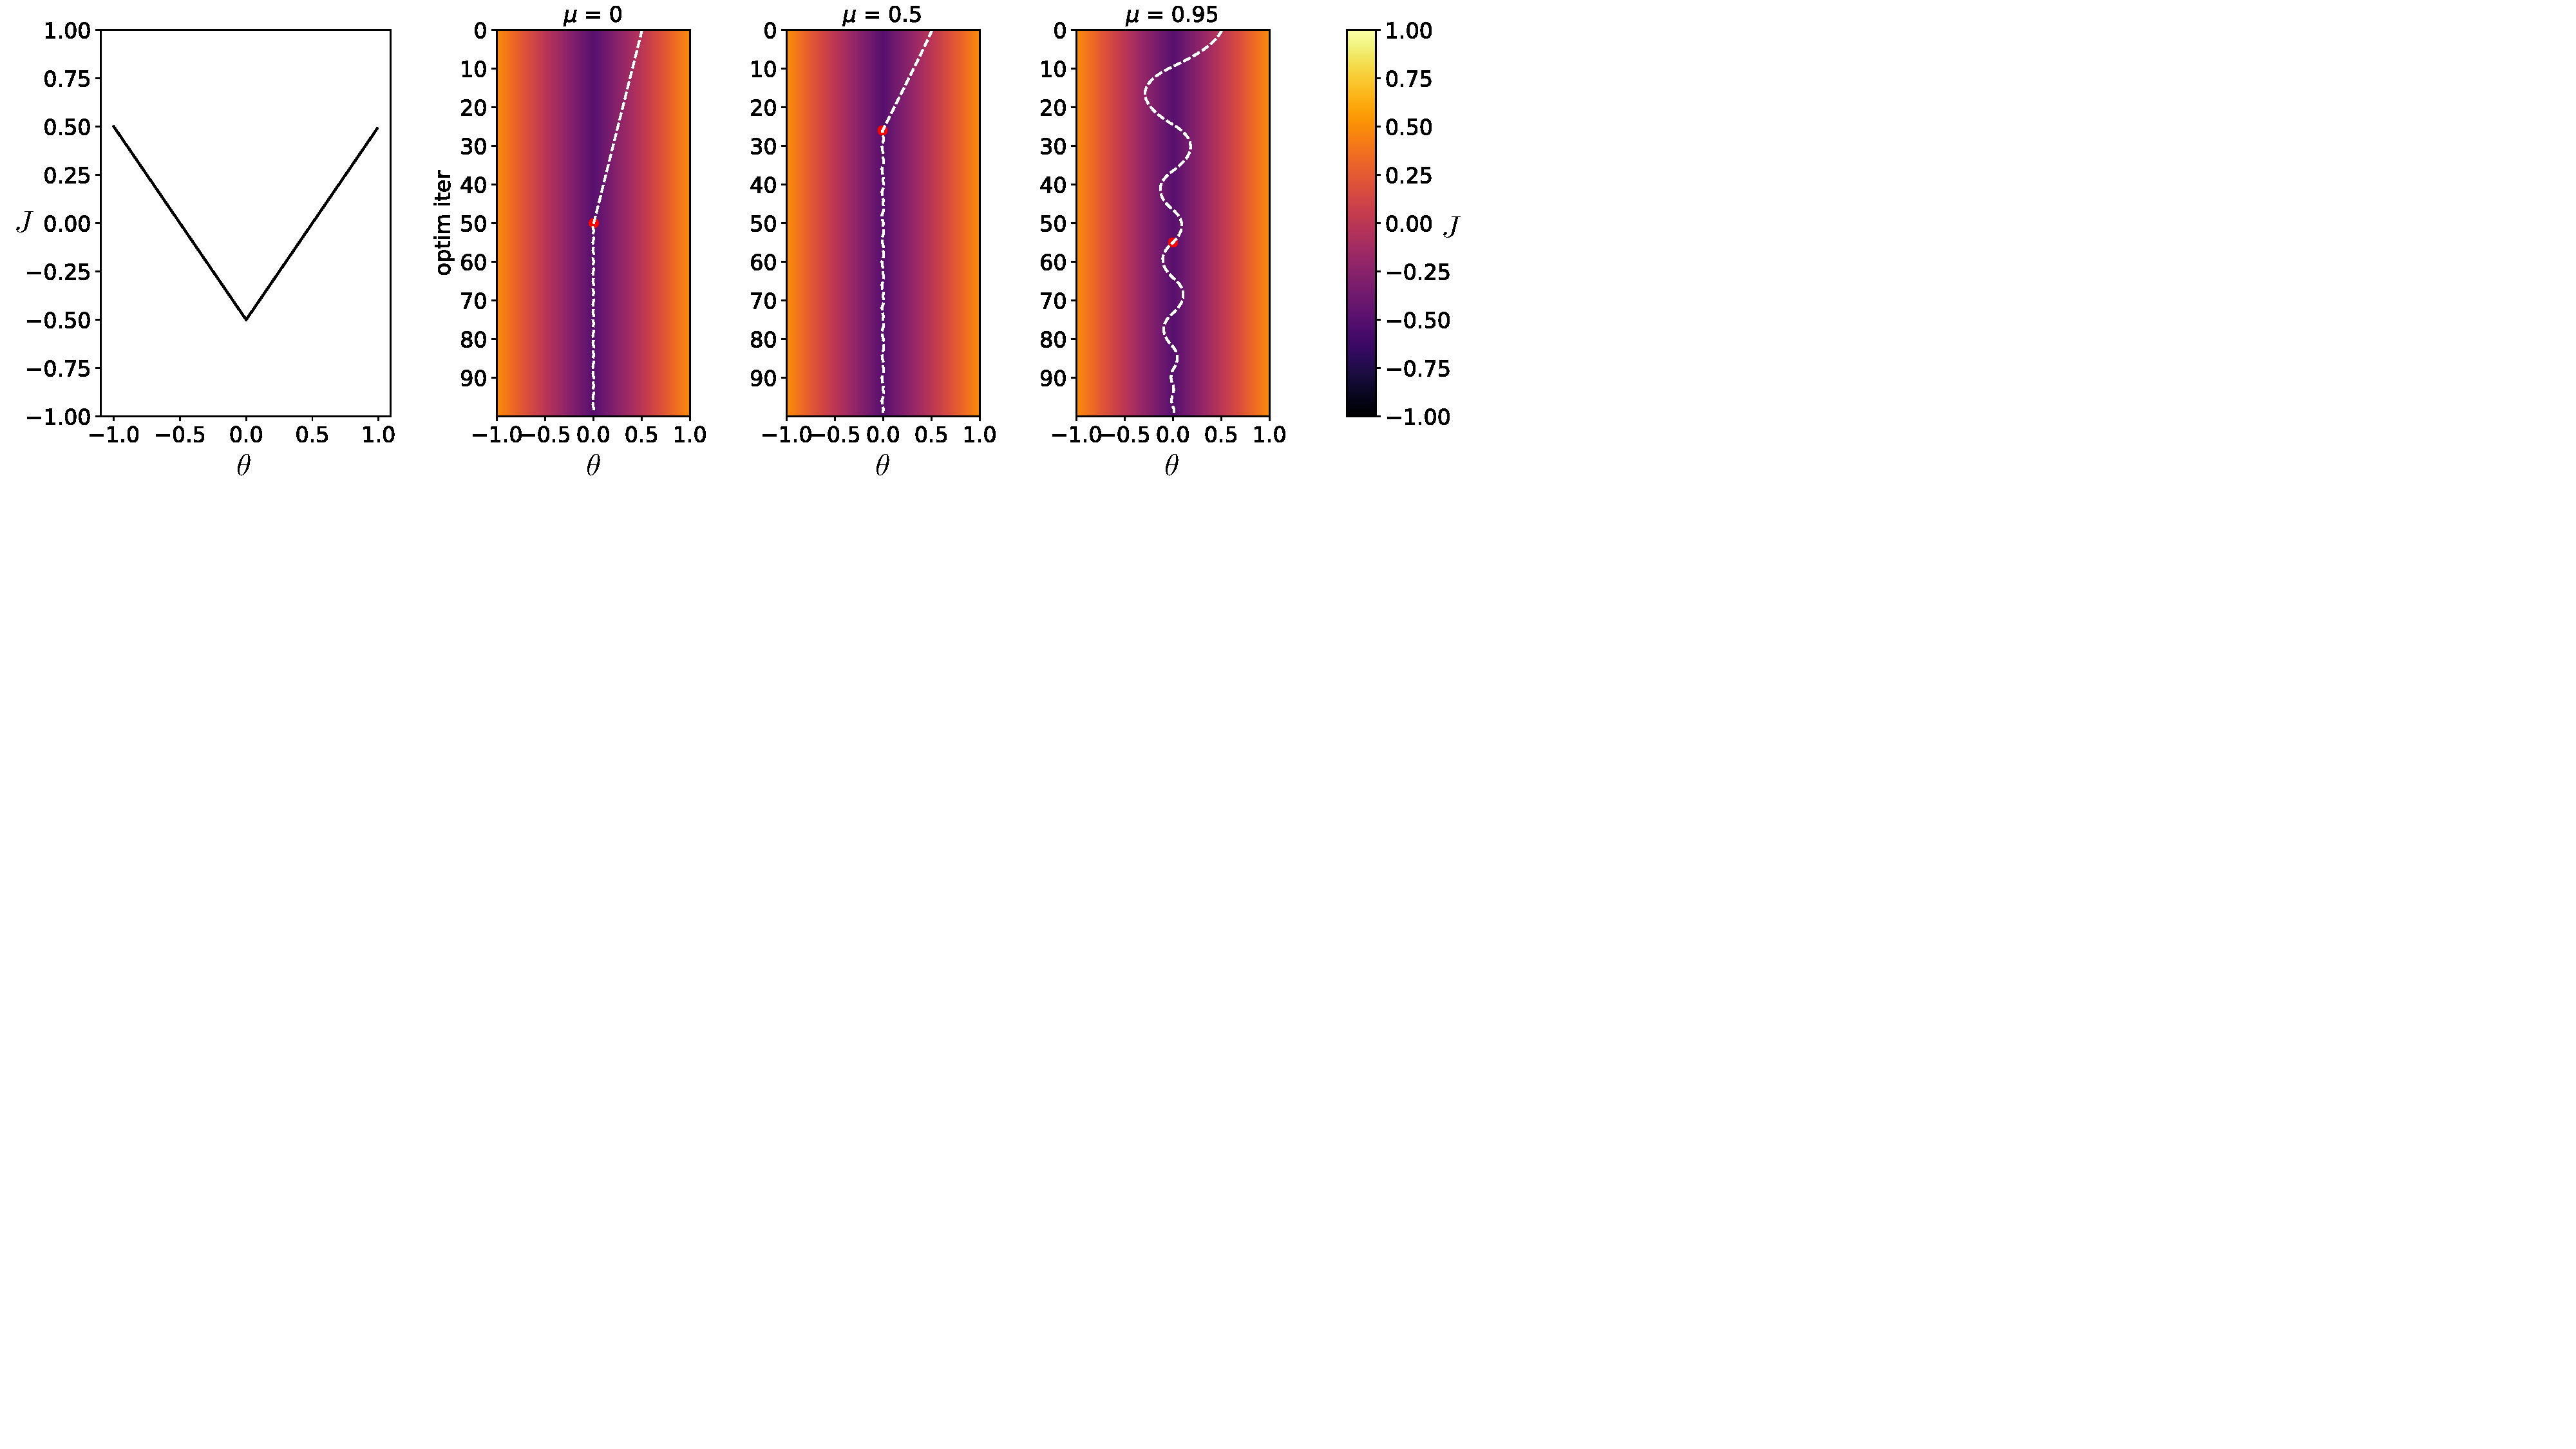
\includegraphics[width=1.0\linewidth]{./figures/gradient_descent/momentum_out1.pdf}
    \caption{(left) A simple loss function $J = \texttt{abs}(\theta)$. (right) Optimization trajectory for three different settings of momentum $\mu$. White line indicates value of the parameter at each iteration of optimization, starting at top and progressing to bottom. Color is value of the loss. Red dot is location where loss first reaches within $0.01$ of optimal value.}
    \label{fig-gradient_descent-momentum_out1}
\end{figure}

It is also possible to come up with other kinds of momentum, which bias the update direction based on some accumulated information from previous updates. Two popular alternatives, which you can read up on elsewhere, are Nesterov's accelerated gradient~\cite{nesterov1983method} and Adam~\cite{kingma2014adam}.


\section{What Kinds of Functions Can Be Minimized with Gradient Descent?}

What if a function is not differentiable? Can we still use gradient descent? Sometimes! The property we need is that we can get a meaningful signal as to how to perturb the function's parameters in order to reduce the loss. This property is \textit{not} the same as differentiability defined in math textbooks. A function may be differentiable but not give useful gradients (e.g., if the gradient is zero everywhere), and a function may be nondifferentiable (at certain points) but still allow for meaningful gradient-based updates (e.g., \texttt{abs}).

\Fig{\ref{fig-gradient_descent-grad_descent_simple_examples}} gives examples of different types of functions being minimized with gradient descent. \Figs{\ref{fig-gradient_descent-grad_descent_simple_examples}}(b) and \ref{fig-gradient_descent-grad_descent_simple_examples}(d) are cases where the function is discontinuous, and the analytical derivative is undefined at the discontinuity. Surprisingly, in \fig{\ref{fig-gradient_descent-grad_descent_simple_examples}}(b), this is not a problem for gradient descent. This is because the gradient descent algorithm we are using here (the one used by Pytorch~\cite{paszke2019pytorch}) uses a \index{One-sided derivative}\textbf{one-sided derivative} at the discontinuity, that is, we set the gradient at the discontinuity to be equal to the gradient value an infinitesimal step away from the discontinuouity in a fixed arbitrary direction. Under the hood, for each atomic discontinuous operation, Pytorch requires that we define its gradients at the discontinuouities, and the one-sided gradient is a standard choice. This is why it can be fine in deep learning (\chap{\ref{chapter-neural_nets}}) to use functions like rectified nonlinear units (relus), which are common in deep networks and have discontinuous gradients.

\Figs{\ref{fig-gradient_descent-grad_descent_simple_examples}}(c) and (e) give cases where the function is continuous, but the gradients are not well-behaved. In \fig{\ref{fig-gradient_descent-grad_descent_simple_examples}}(c) we have a gradient that has nearly \index{Vanishing gradient}\textbf{vanished}, that is, it is near zero everywhere and gradient descent, with a fixed learning rate, will therefore be slow. \Fig{\ref{fig-gradient_descent-grad_descent_simple_examples}}(e) shows the opposite scenario: the gradient at the minimizer goes to infinity; we call this an \index{Exploding gradient}\textbf{exploding gradient}, and this leads to failures of convergence. 

Finally, \fig{\ref{fig-gradient_descent-grad_descent_simple_examples}}(f) shows one more problematic case: when there are multiple minima, gradient descent can get stuck in a suboptimal minimum. Which minimum we arrive at will depend on where we initialized $x$.  

\begin{figure}[h!]
    \centerline{
    \begin{tabular}{cc}
        (a) convex & (b) discontinuous \\
        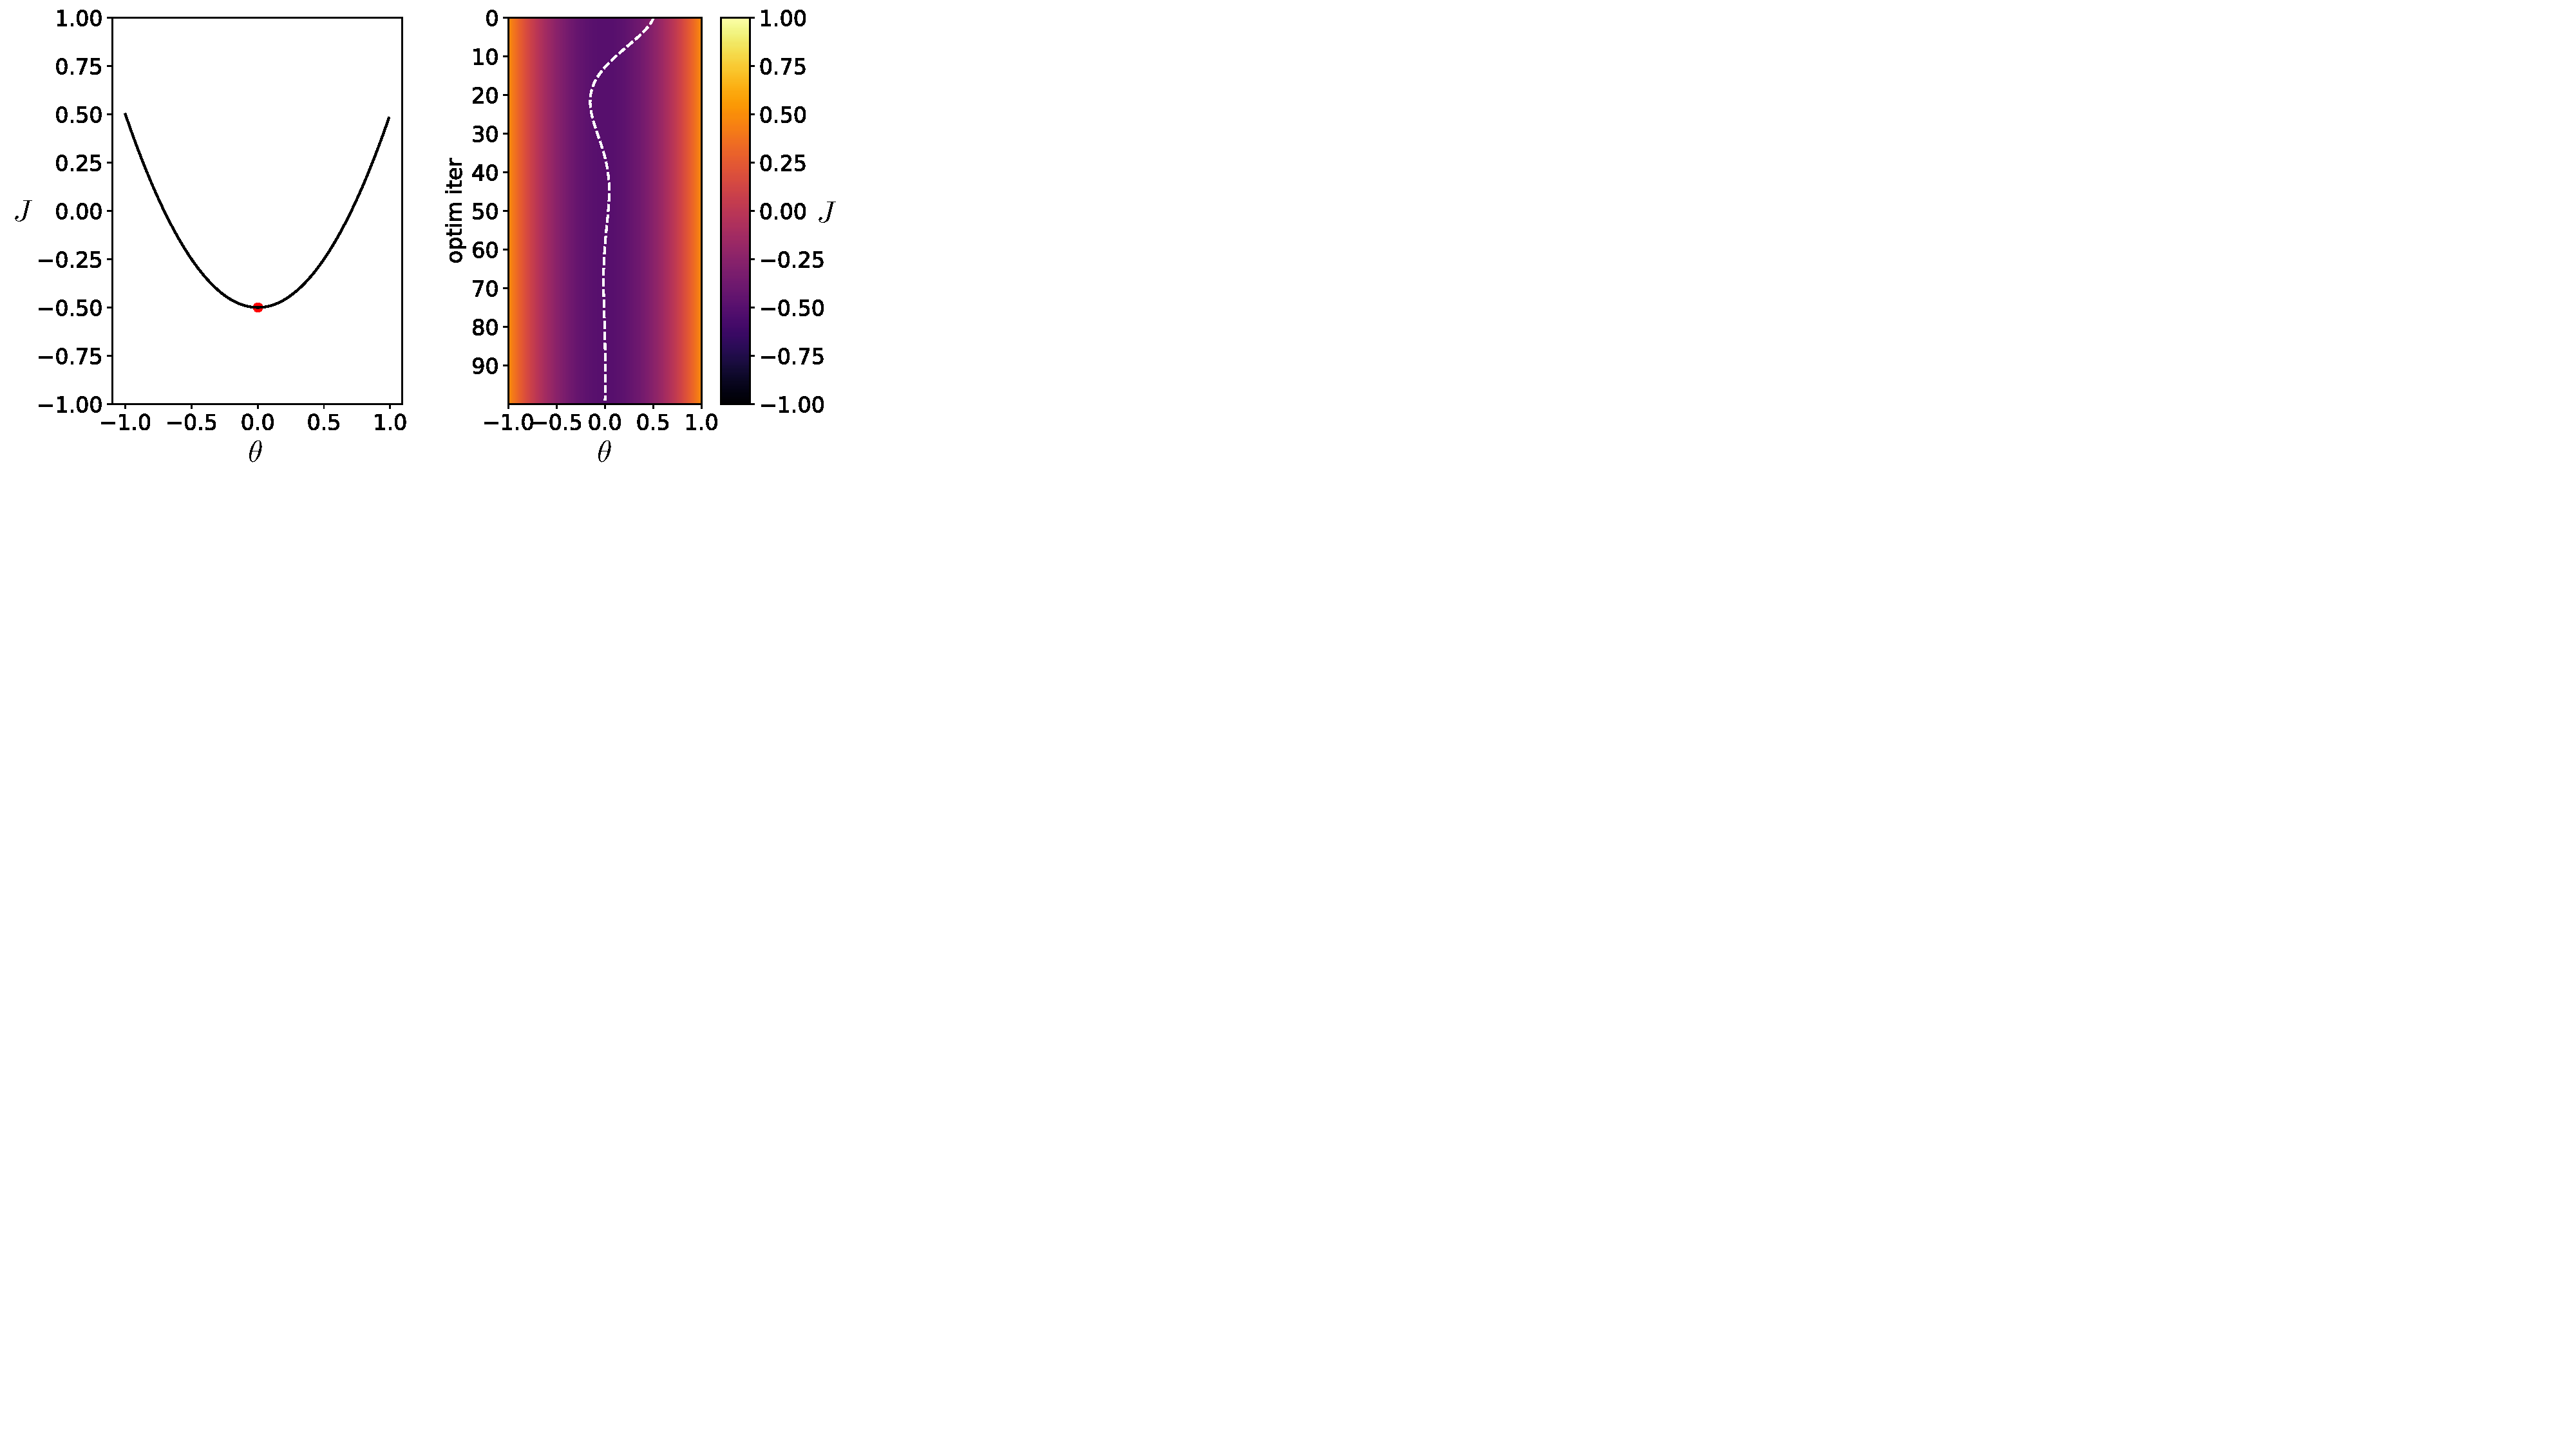
\includegraphics[width=0.5\linewidth]{./figures/gradient_descent/grad_descent_ex1.pdf} & 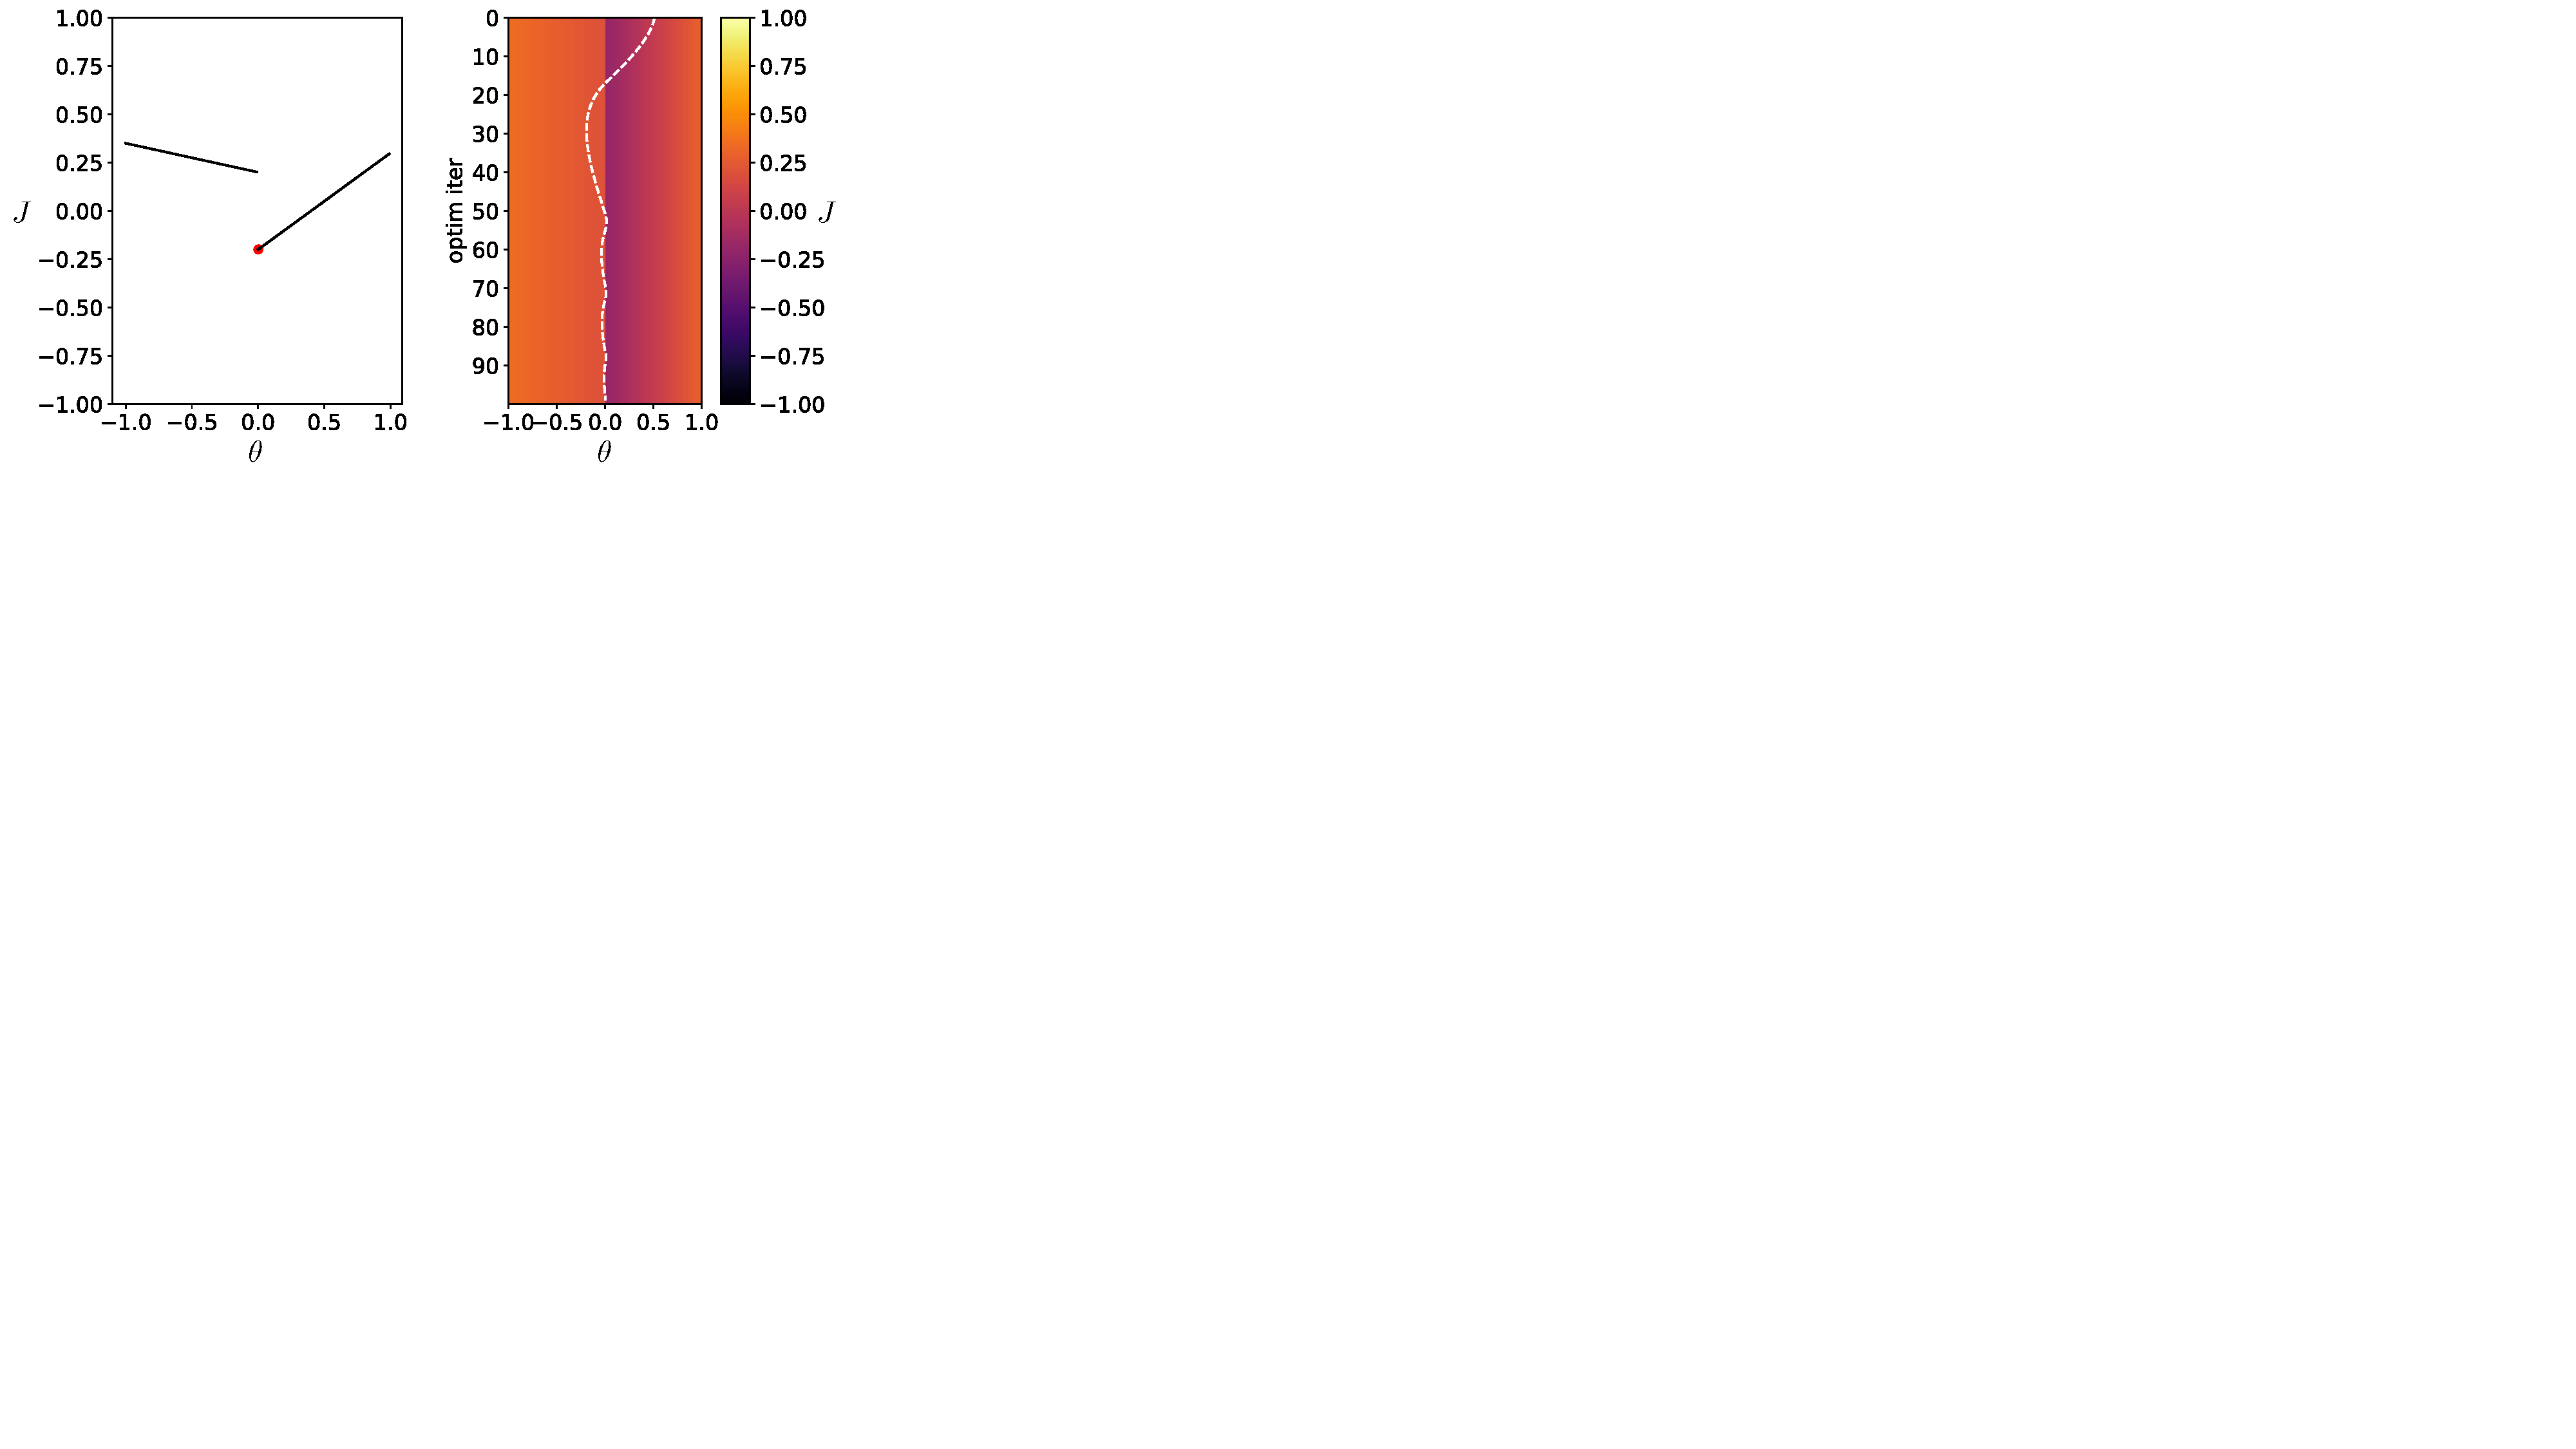
\includegraphics[width=0.5\linewidth]{./figures/gradient_descent/grad_descent_ex2.pdf} \\
        (c) vanishing gradient & (d) zero gradient + discontinuous \\
        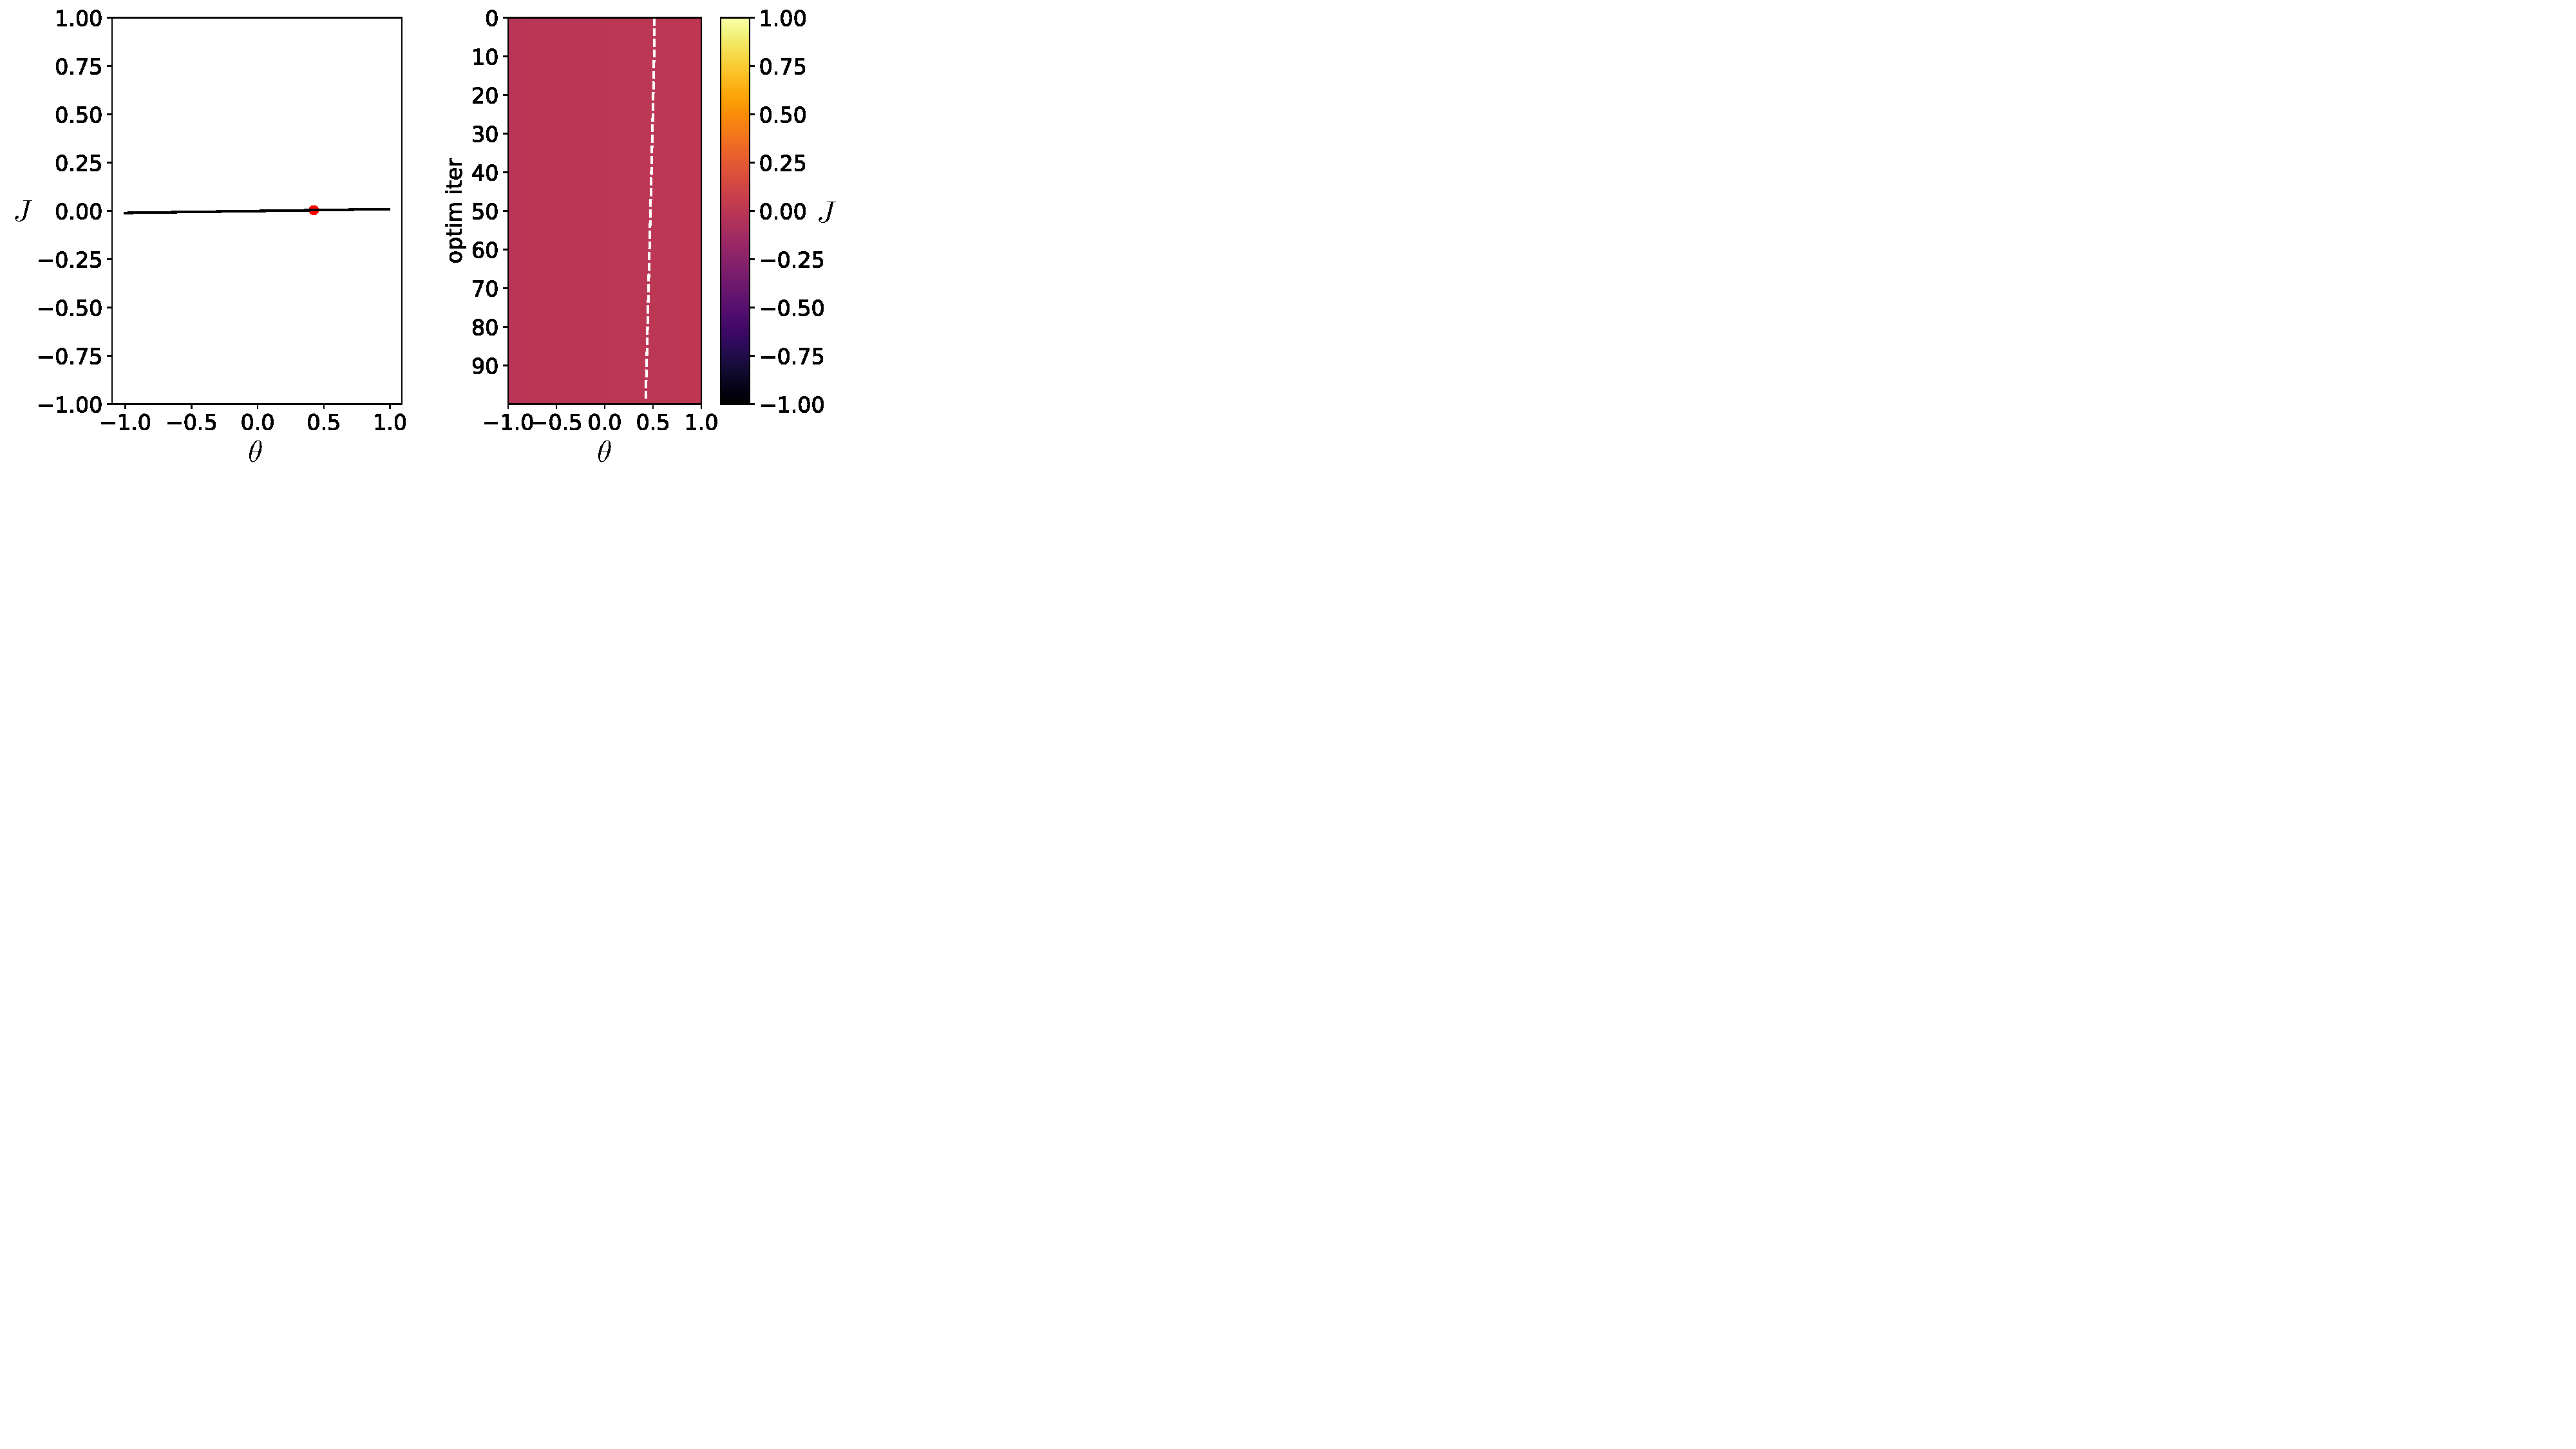
\includegraphics[width=0.5\linewidth]{./figures/gradient_descent/grad_descent_ex4.pdf} &
        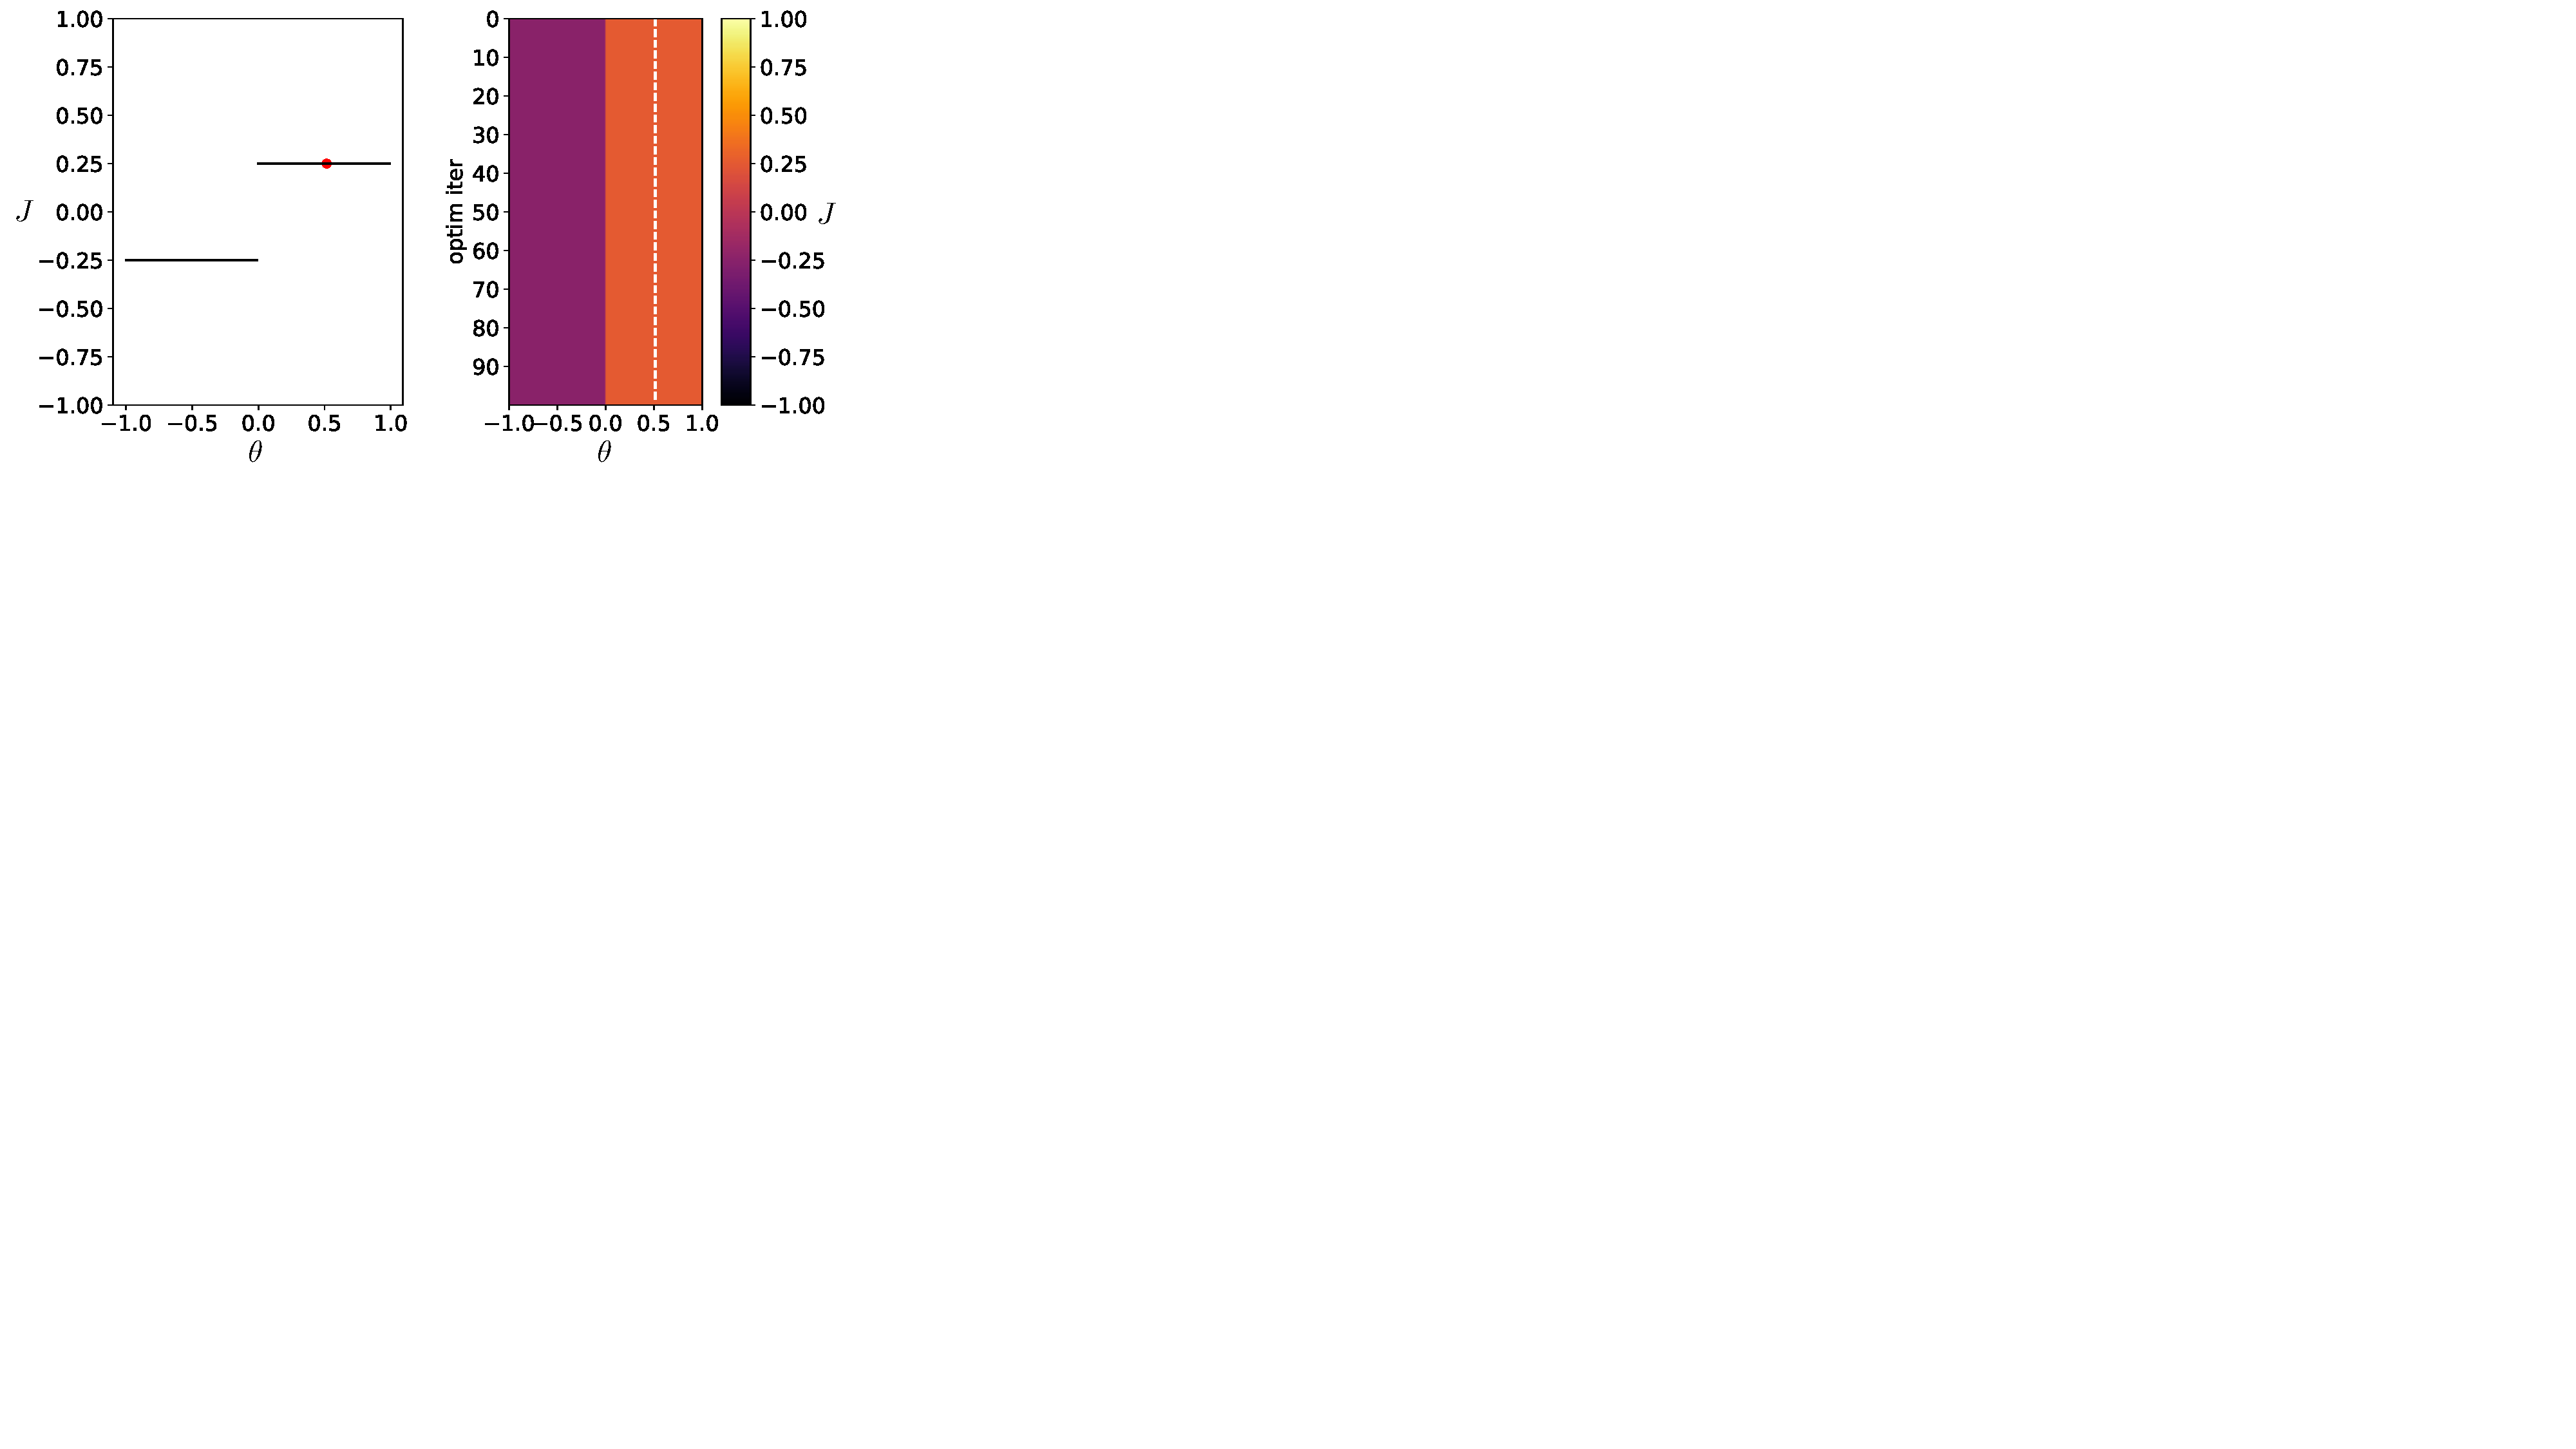
\includegraphics[width=0.5\linewidth]{./figures/gradient_descent/grad_descent_ex3.pdf} \\
        (e) exploding gradient & (f) multiple local minima \\
        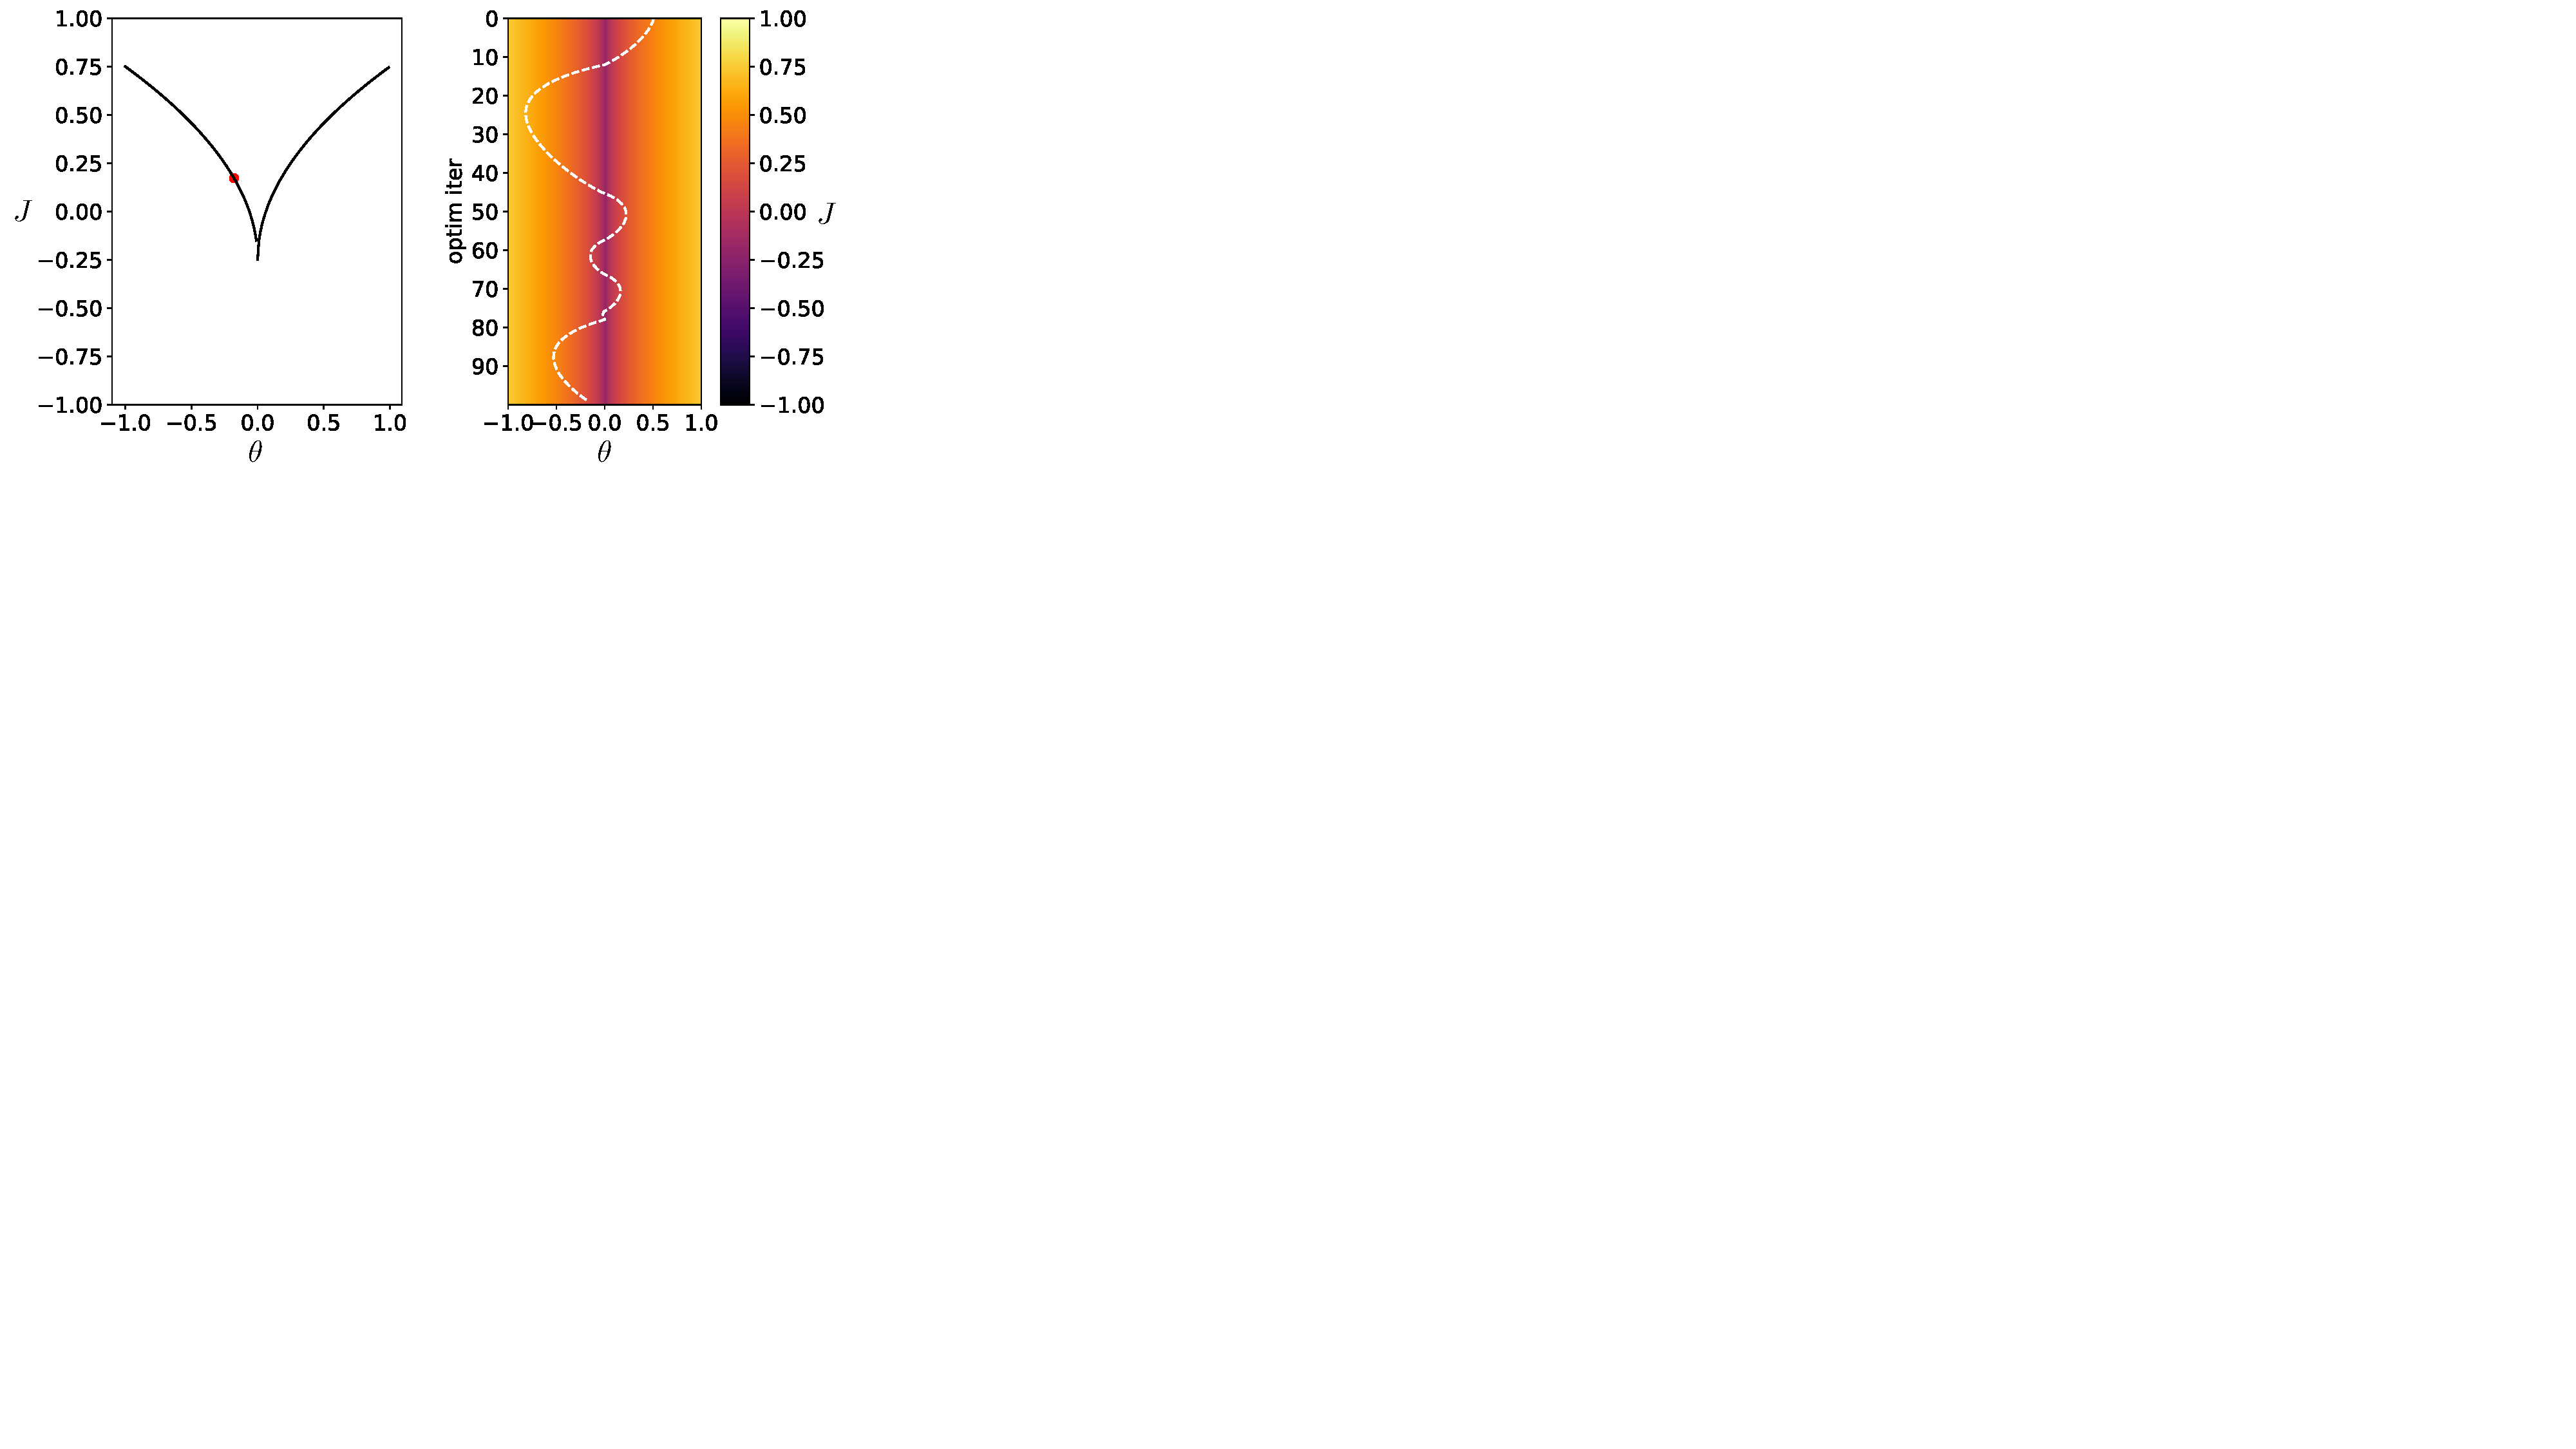
\includegraphics[width=0.5\linewidth]{./figures/gradient_descent/grad_descent_ex5.pdf} & 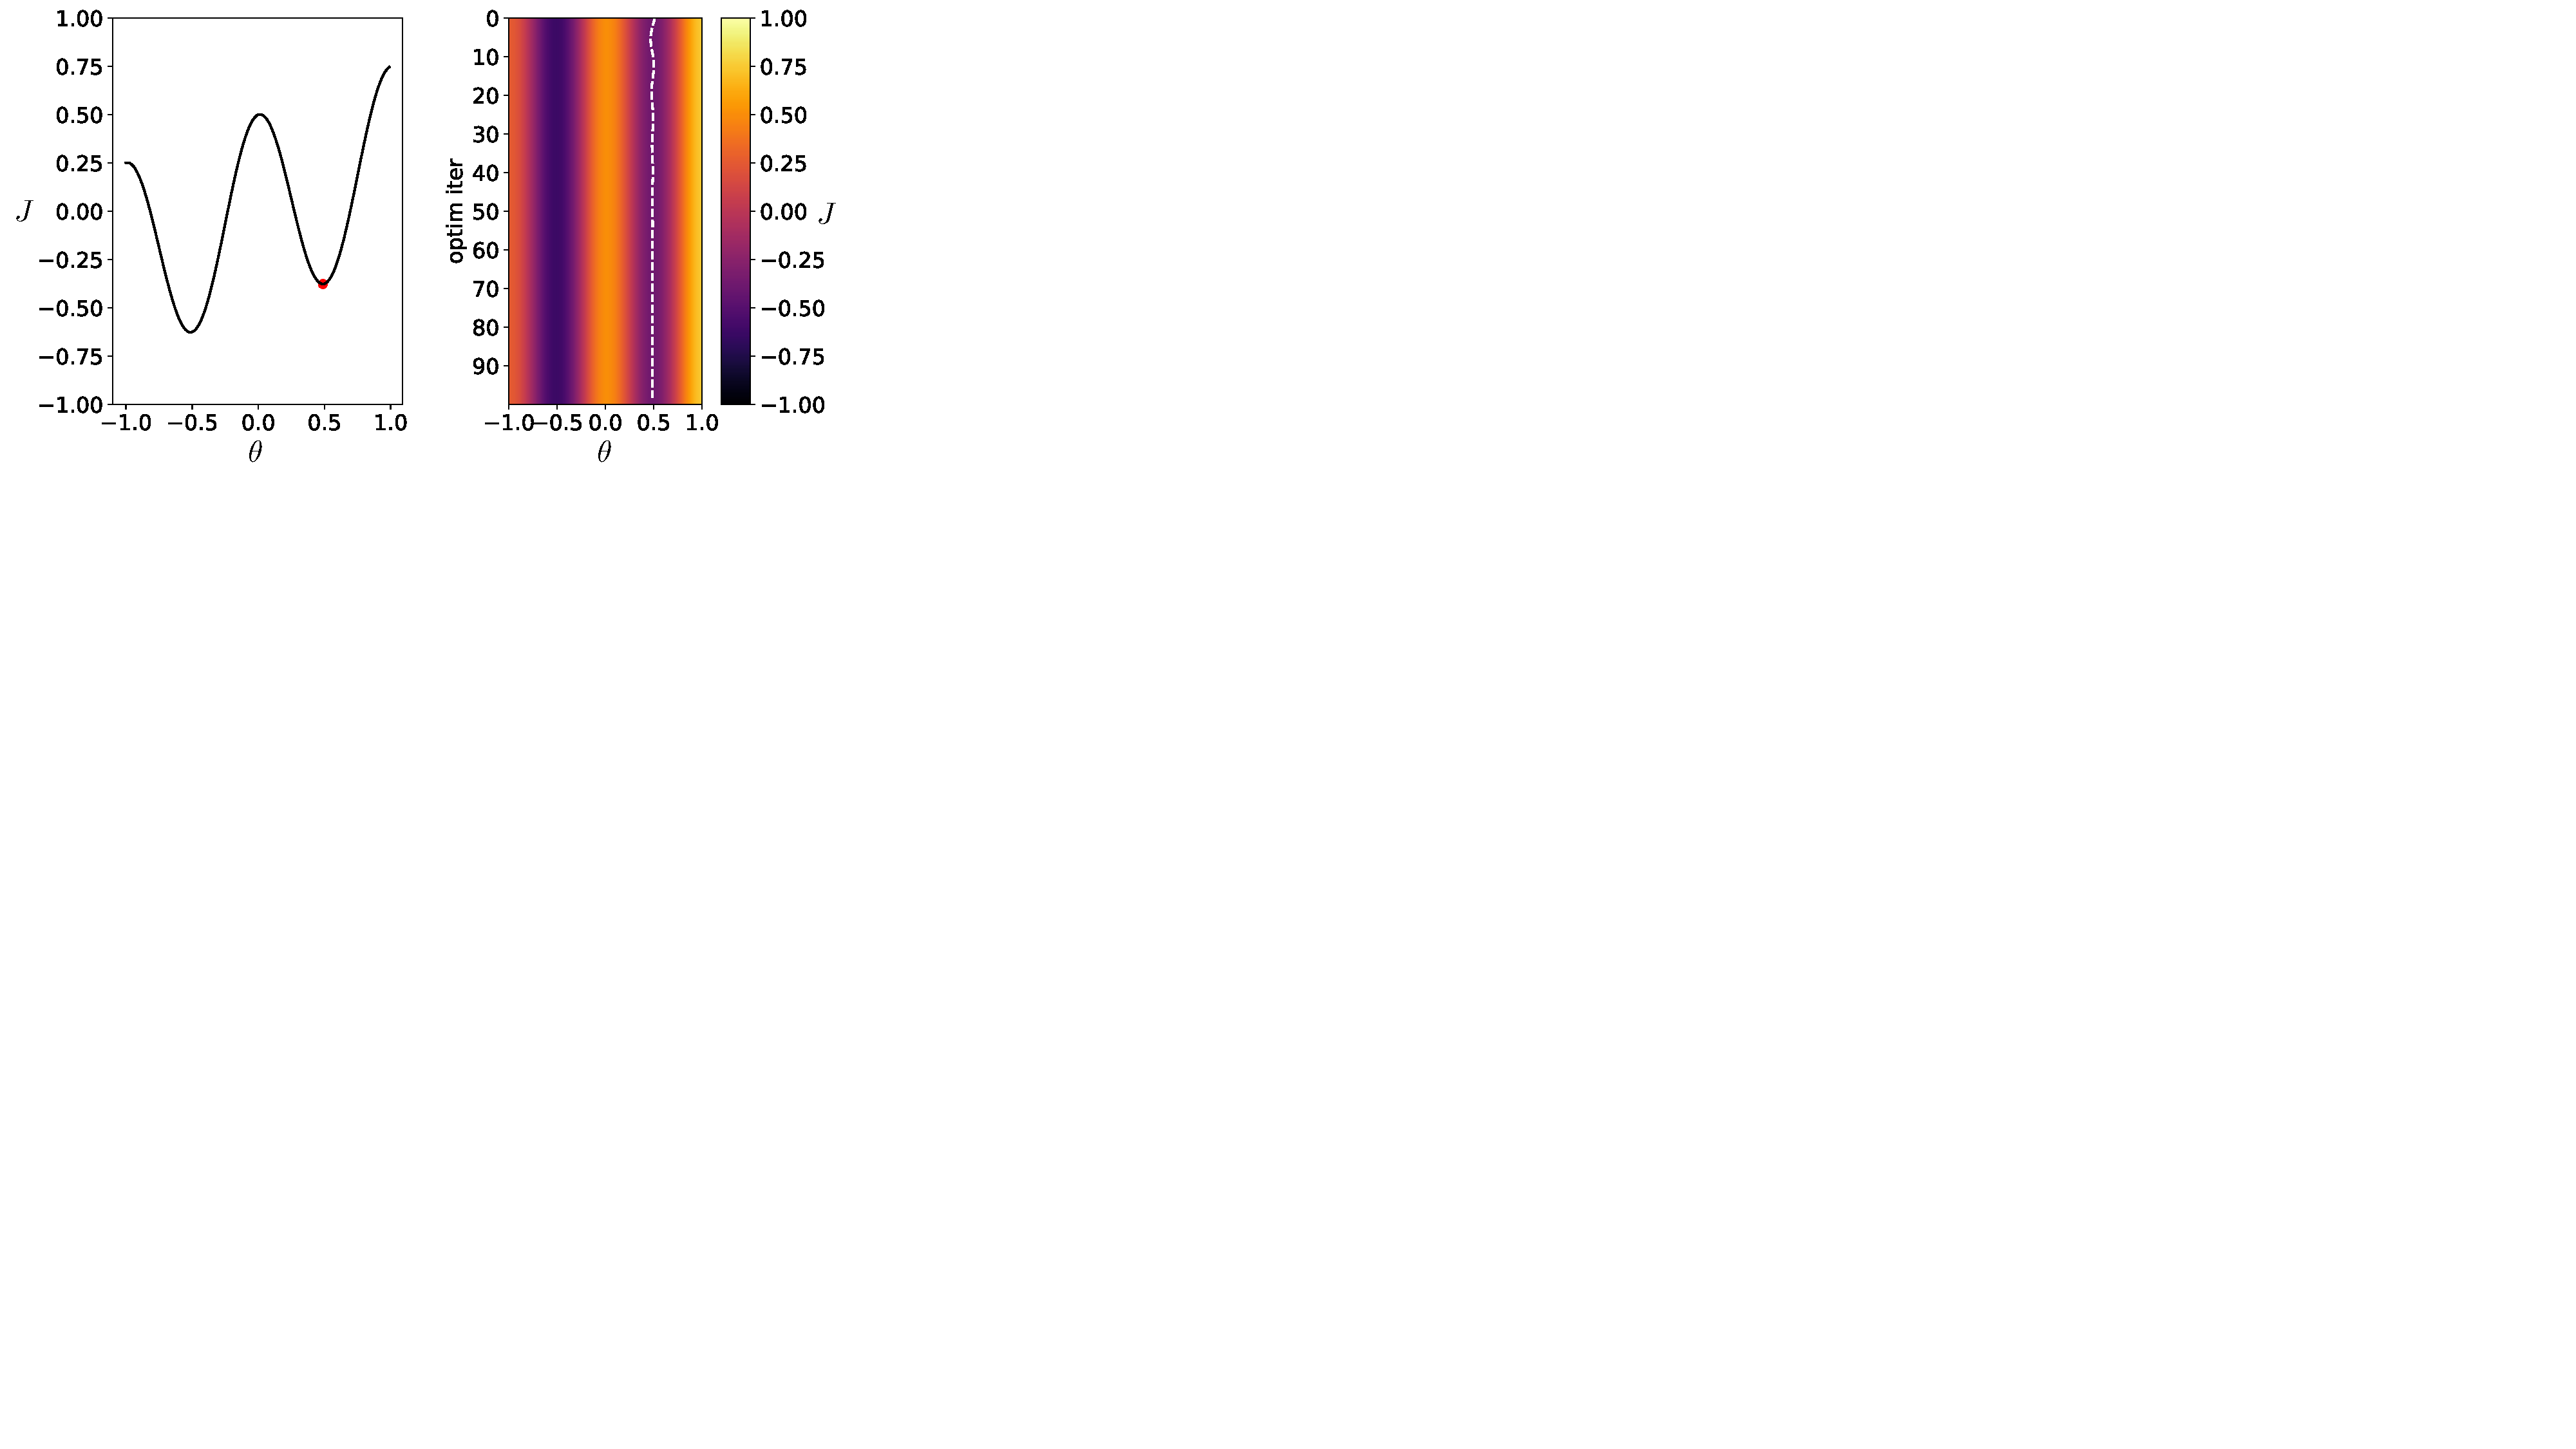
\includegraphics[width=0.5\linewidth]{./figures/gradient_descent/grad_descent_ex6.pdf}
    \end{tabular}
    }
    \caption{How gradient descent behaves on various functions. In each subplot, left is the function $J$, the red point is the solution found by $\GD$ (with $\eta=0.01$ and $\mu=0.9$), and right is the trajectory of $x$ values over iterations of $\GD$, plotted on top of $J$ at each iteration. (a) As $\eta$ goes to zero, $\GD$ converges for convex functions. (b) Discontinuities pose no essential problem, as long as the gradient is defined on either side. (c) A nearly flat function will exhibit very slow descent. (d) Piecewise constant functions are problematic because the gradient completely vanishes. (e) For the function $J=\texttt{sqrt}(\texttt{abs}(\theta))-0.25$, the gradient goes to infinity at the minimizer, causing instability. (f) When $J$ has multiple local minima, we may not find the global minimum.}
    \label{fig-gradient_descent-grad_descent_simple_examples}
\end{figure}


\subsection{Gradient-Like Optimization for Functions without Good Gradients}\label{sec-gradient_descent-zeroth_order}
What about minimizing functions like \fig{\ref{fig-gradient_descent-grad_descent_simple_examples}}(d), where the gradient is zero almost everywhere? This is a case where gradient descent truly struggles. However, it is often possible to transform such a problem into one that can be treated with gradient descent. Remember that the key property of a gradient, from the perspective of optimization, is that it is a locally loss-minimizing direction in parameter space. Most gradient-based optimizers don't really need true gradients; instead their update functions are compatible with a broader family of local loss-minimizing directions, $\mathbf{v}$. 

Besides the true gradient, what are some other good choices for $\mathbf{v}$? One common idea is to set $\mathbf{v}$ to be the gradient of a \index{Surrogate loss}\textbf{surrogate loss} function, which is a function, $J_{\texttt{surr}}$, with meaningful (non-zero) gradients, that approximates $J$. An example might be a smoothed version of $J$. Another way to get $\mathbf{v}$ is to compute it by sampling perturbations of $\theta$, and seeing which perturbation leads to lower loss. In this strategy, we evaluate $J(\theta+\epsilon)$ for a set of perturbations $\epsilon$, then move toward the $\epsilon$'s that decreased the loss. Approaches of this kind are sometimes called \index{Evolution strategies}\textbf{evolution strategies}~\cite{beyer2002evolution, salimans2017evolution}, and a basic version of this algorithm is given in \algref{\ref{alg-gradient_descent-ES}}.
%\vspace{-0.5cm}
\begin{algorithm}[h!]
\SetAlgoVlined
\DontPrintSemicolon
%\marginnote{{\bf Algorithm \ref{alg-gradient_descent-ES}}: Optimizing a cost function $J: \theta \rightarrow \mathbb{R}$ by evolution strategies, i.e., sampling different values for $\theta$ and taking a step toward the values that work best.}
\caption{{\bf Algorithm \ref{alg-gradient_descent-ES}}: Evolution strategies (\texttt{ES}). Optimizing a cost function $J: \theta \rightarrow \mathbb{R}$ by evolution strategies, i.e., sampling different values for $\theta$ and taking a step toward the values that work best.}
\fakealgorithmcaption{}
\label{alg-gradient_descent-ES}
{\bf Input:} objective function $J$, initial parameter vector $\theta^0$, learning rate $\eta$, sampling standard deviation $\sigma$, number of samples $M$, number of steps $K$\;%, data $\{\mathbf{x}^{(i)},\mathbf{y}^{(i)}\}_{i=1}^N$
{\bf Output:} trained parameter vector $\theta^* = \theta^K$\;
\For{\upshape $k= 0, \dots, K-1$}{
    \For{\upshape $i= 1, \dots, M$}{
        $\epsilon_i \sim \mathcal{N}(\mathbf{0},\mathbf{I})$\;
        $s_i = J(\theta + \sigma \epsilon_i)$\;
    }
    $\theta^{k+1} \leftarrow \theta^{k} - \eta \frac{1}{\sigma M}\sum^M_{i=1} s_i \epsilon_i$\;
}
\end{algorithm}
%\vspace{-0.5cm}

As shown in \fig{\ref{fig-gradient_descent-sampling_out1}}, this algorithm can successfully minimize the function in \fig{\ref{fig-gradient_descent-grad_descent_simple_examples}}(c).
\begin{figure}[h!]
    %\vspace{-0.75cm}
    \centerline{
    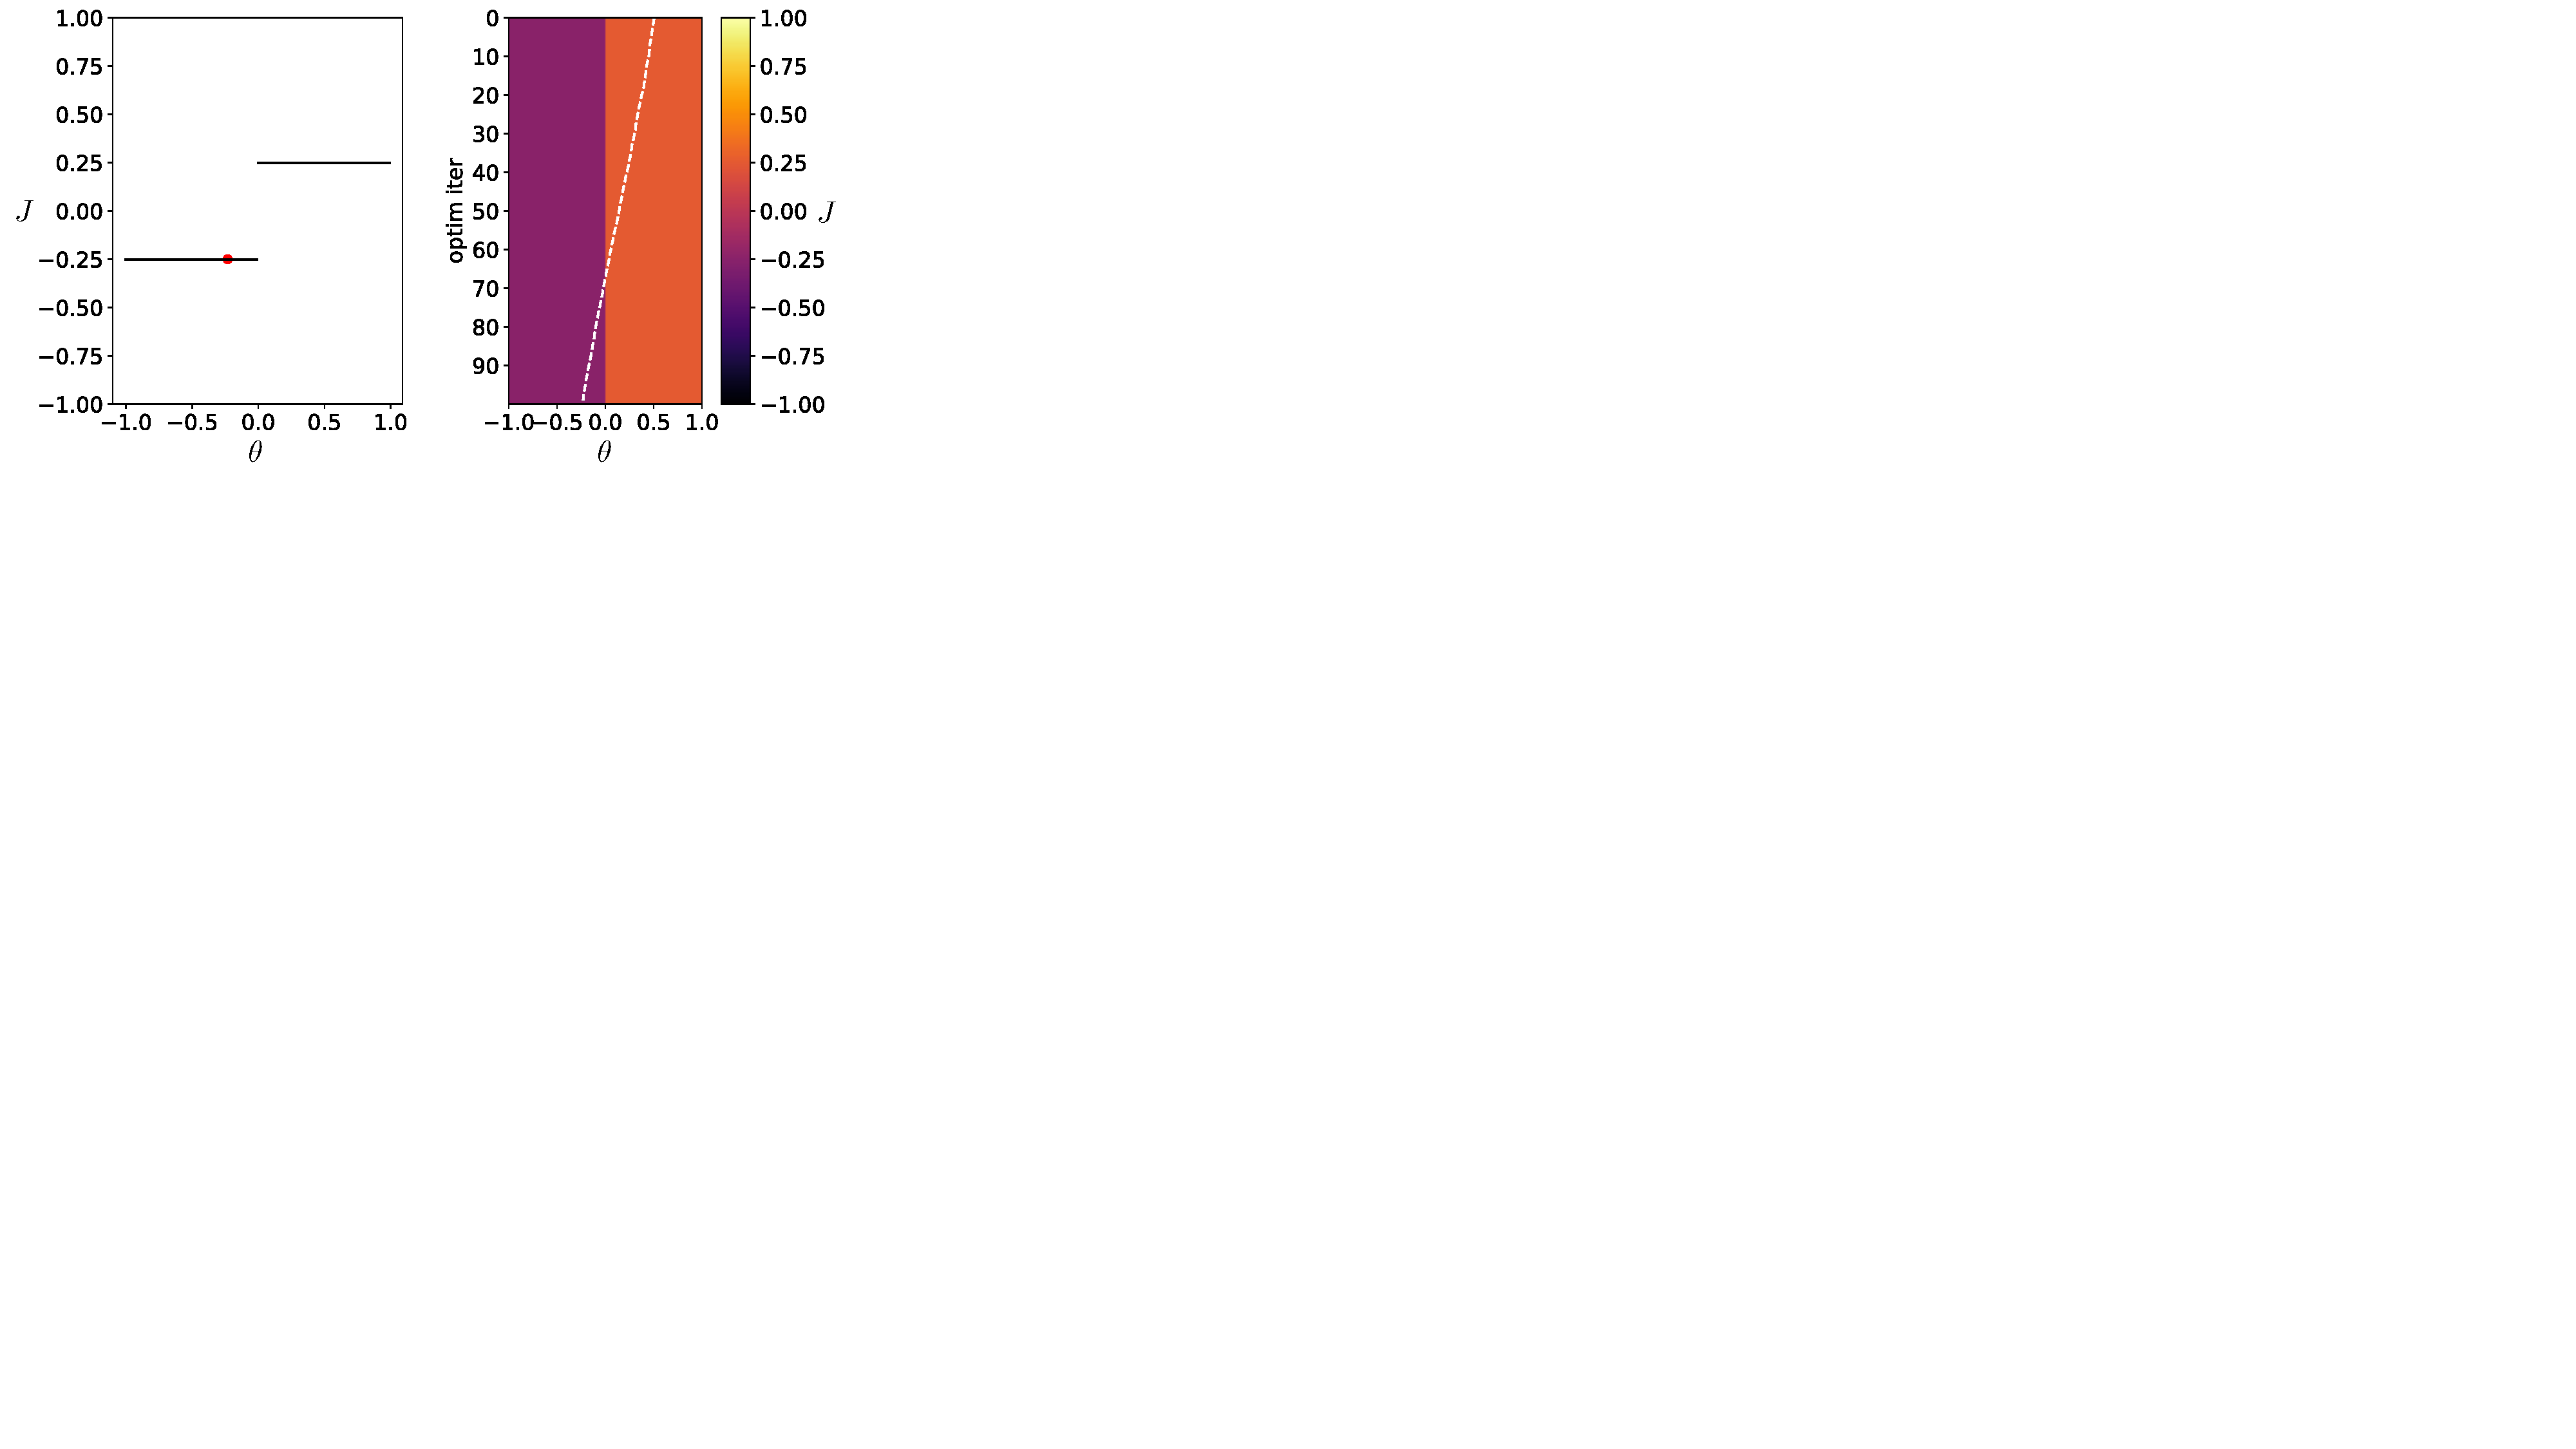
\includegraphics[width=0.5\linewidth]{./figures/gradient_descent/sampling_out1.pdf}
    }
    \caption{Using \ES~(\algref{\ref{alg-gradient_descent-ES}}) to minimize a nondifferentiable (zero-gradient) loss, using $\sigma=1$, $M=10$, and $\eta=0.02$.}
    \label{fig-gradient_descent-sampling_out1}
    %\vspace{-0.75cm}
\end{figure}

\subsection{Gradient Clipping}
What about \fig{\ref{fig-gradient_descent-grad_descent_simple_examples}}(e), where the gradient explodes near the optimum? Is there anything we can do to improve optimization of this function? To combat exploding gradients, a useful trick is \index{Gradient clipping}\textbf{gradient clipping}, which just means clamping the magnitude of the gradient to some maximum value. \Algref{\ref{alg-gradient_descent-grad_clipping}} describes this approach.

\begin{algorithm}[h]
\SetAlgoVlined
\DontPrintSemicolon
%\marginnote{{\bf Algorithm \ref{alg-gradient_descent-grad_clipping}}: Gradient descent with gradient clipping.}
\caption{{\bf Algorithm \ref{alg-gradient_descent-grad_clipping}}: Gradient descent with gradient clipping.}
\fakealgorithmcaption{}
\label{alg-gradient_descent-grad_clipping}
{\bf Input:} objective function $J$, initial parameter vector $\theta^0$, learning rate $\eta$, number of steps $K$, max gradient magnitude $m$\;%, data $\{\mathbf{x}^{(i)},\mathbf{y}^{(i)}\}_{i=1}^N$
{\bf Output:} trained parameter vector $\theta^* = \theta^K$\;
\For{\upshape $k= 0, \dots, K-1$}{
    %$J = \sum_{i=1}^N \mathcal{L}(f_{\theta^{k-1}}(\mathbf{x}^{(i)}),\mathbf{y}^{(i)})$\;
    $\mathbf{v} = \nabla_{\theta} J(\theta^k)$\;
    %$\theta^{k+1} \leftarrow \theta^{k} - \eta %[\max(\min(v_1,m),-m),\ldots,\max(\min(v_M,m),-m)]^\transpose$\; %\quad\quad \triangleleft \text{per-dimension clipping}$\;
    %$\theta^{k} \leftarrow \theta^{k-1} - \eta \min(\norm{\mathbf{v}},m)\frac{\mathbf{v}}{\norm{\mathbf{v}}}$\;
     $\theta^{k+1} \leftarrow \theta^{k} - \eta [\texttt{clip}(v_1, -m, m), \ldots, \texttt{clip}(v_M, -m, m)]^\transpose$
}
\end{algorithm}
\marginnote{\texttt{clip} is the ``clipping'' function: $\texttt{clip}(v, -m, m) = \max(\min(v,m),-m)$}[-1.6cm]

This algorithm indeed successfully minimizes our example of the exploding gradient, as can be seen in \fig{\ref{fig-gradient_descent-clipped_out1}}.
\begin{figure}[h]
    \centerline{
    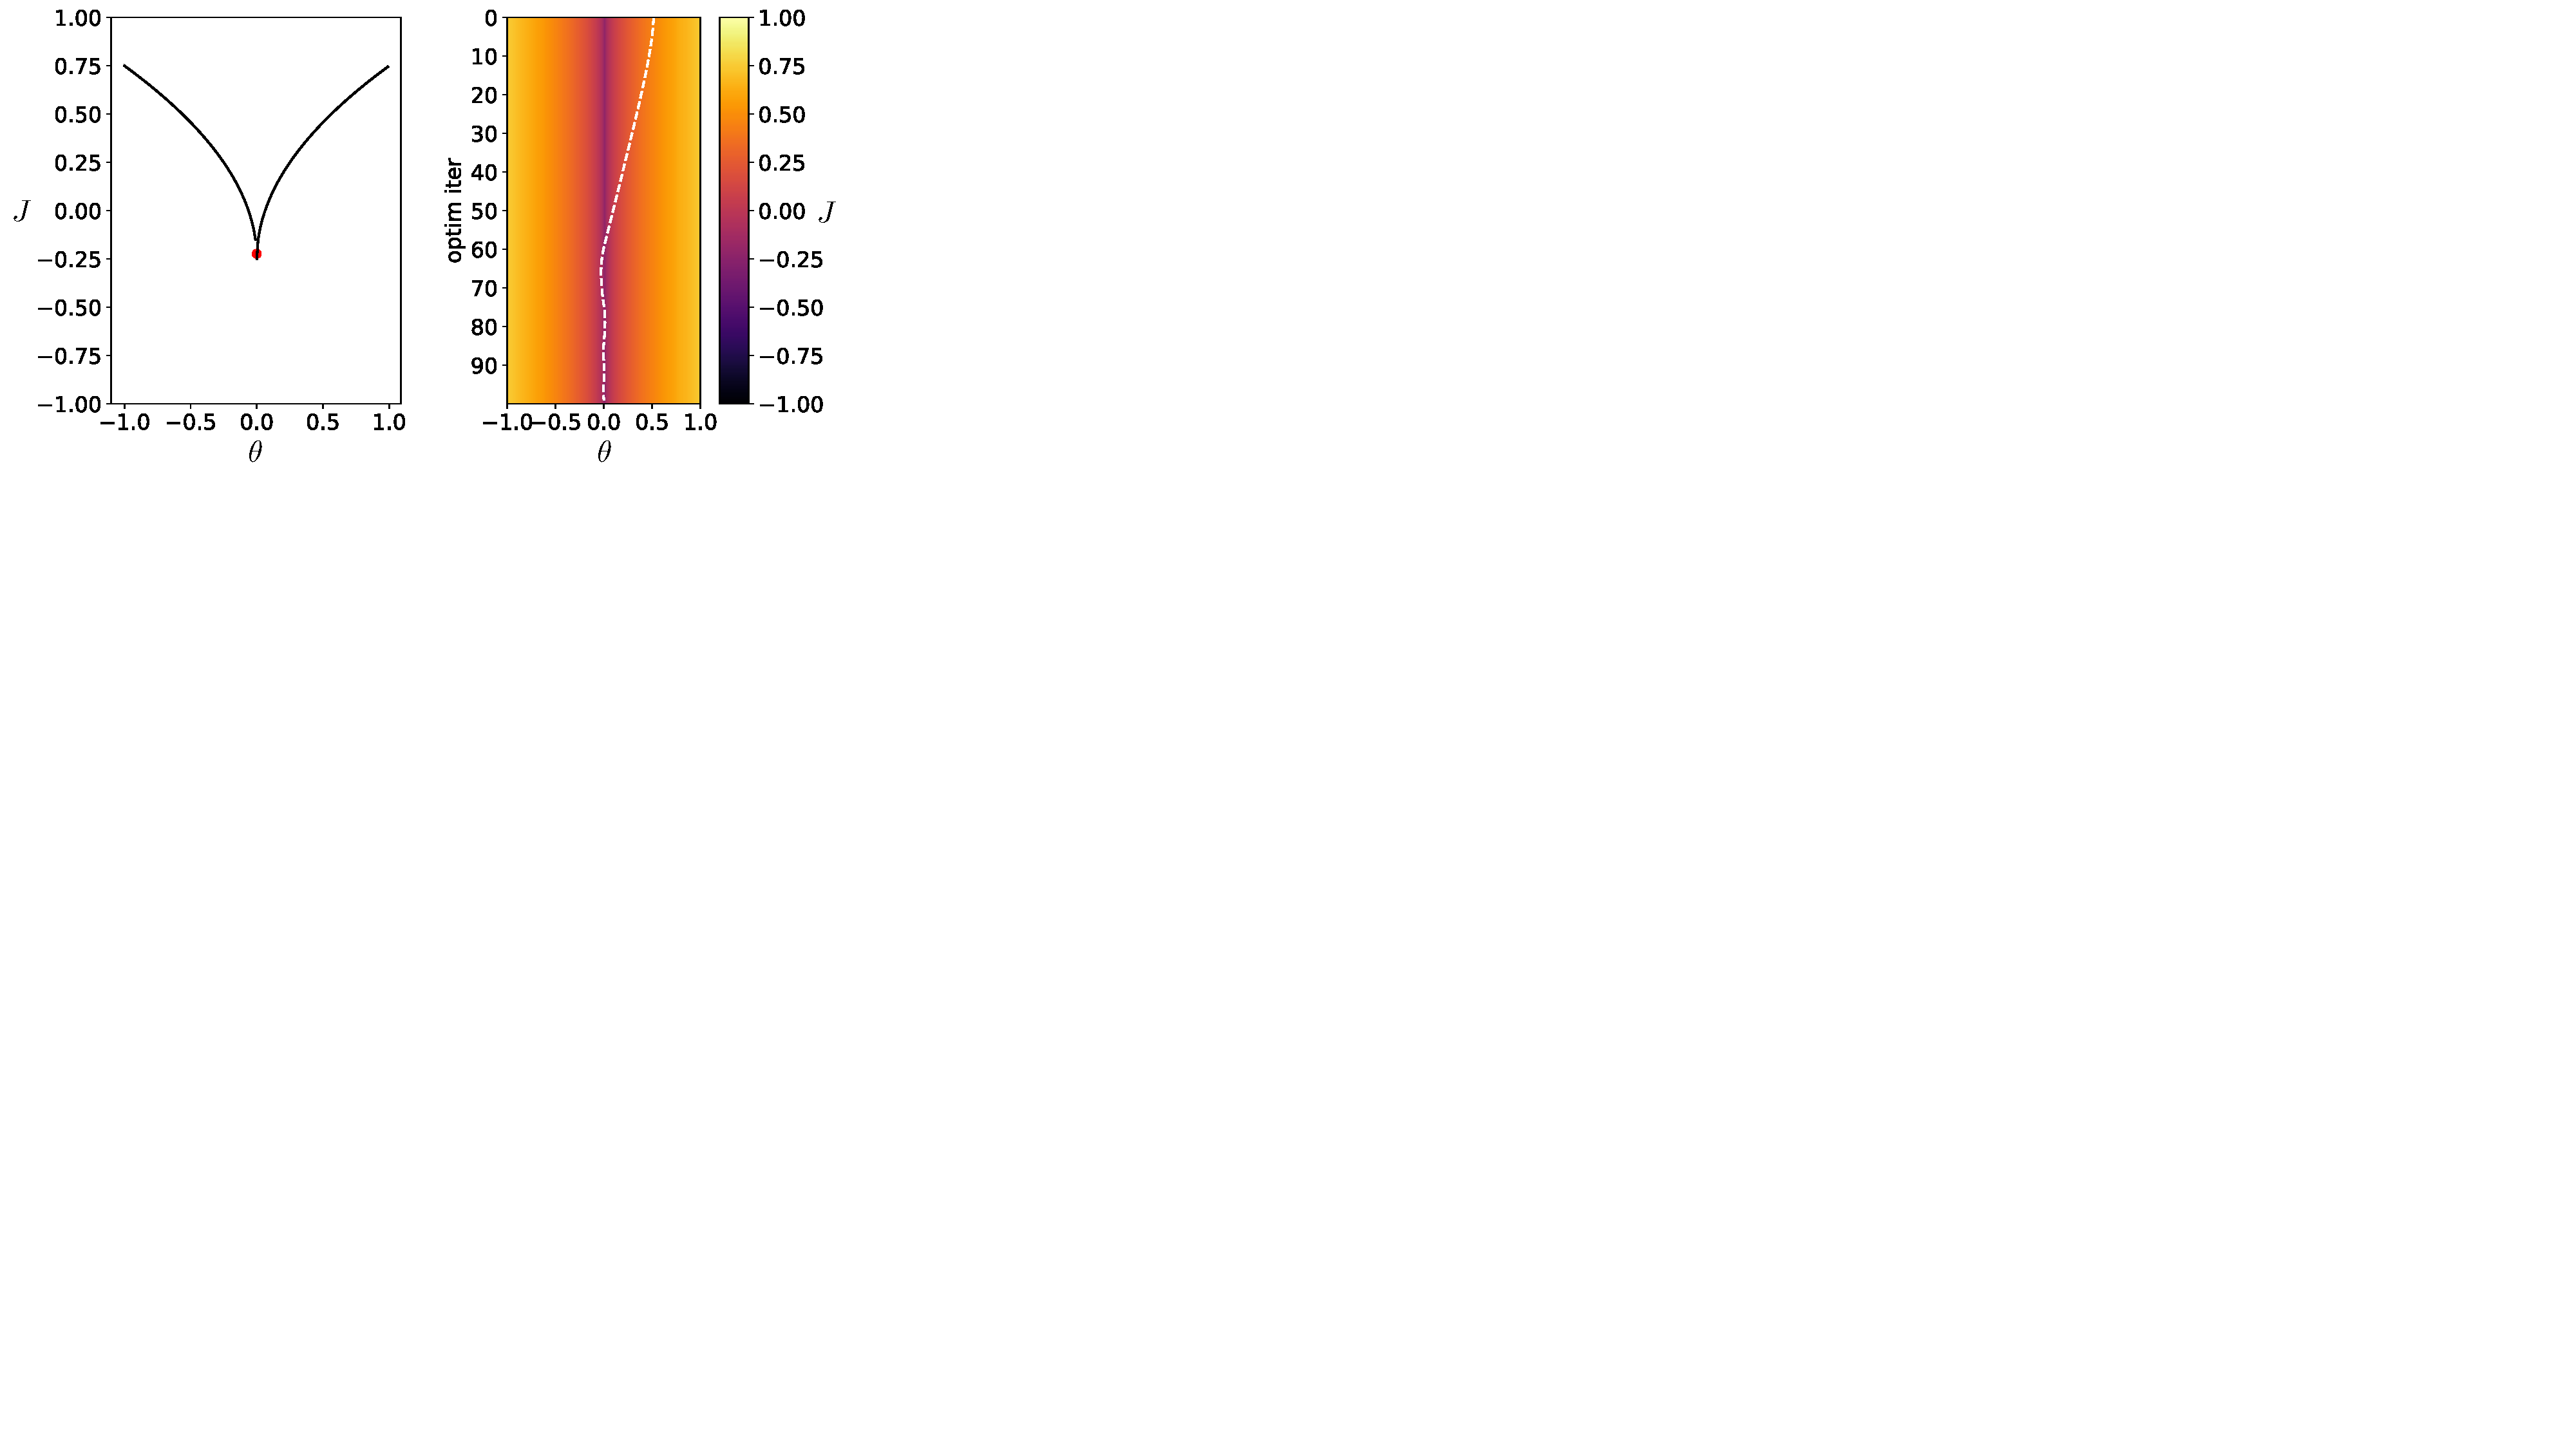
\includegraphics[width=0.5\linewidth]{./figures/gradient_descent/clipped_out1.pdf}
    }
    \caption{Using \GD~with clipping to minimize a loss with exploding gradients, using $m=0.1$.}
    \label{fig-gradient_descent-clipped_out1}
\end{figure}

%This is a case where gradient descent truly struggles. However, with a small modification, gradient descent again becomes applicable. The modification is to descend the gradient of a smooth approximation to $J$, which we will call $J_{\texttt{smooth}}$, rather than to $J$ itself. Given some data, we can either \textit{globally} fit $J_{\texttt{smooth}}$ to $J$, then plug $J_{\texttt{smooth}}$ into Algorithm \ref{alg-gradient_descent-basic_gradient_descent}, or we can proceed in an ``online" fashion, where on each iteration of gradient descent, we \textit{locally} compute: just for this operating point what is the smooth gradient? The latter can be more efficient since we only have to do the approximation for the operating points we visit, which may be a very small subspace of the total parameter space. For this approach, in practice, on each iteration of gradient, we may sample \textbf{finite differences} to find the locally linear approximation to the loss surface:

%The property that we need is that at each operating point, a loss-minimizing direction, $\mathbf{v}$, can given as the input to the update function. This gradient 

% \begin{figure}[h]
%     \centering
%     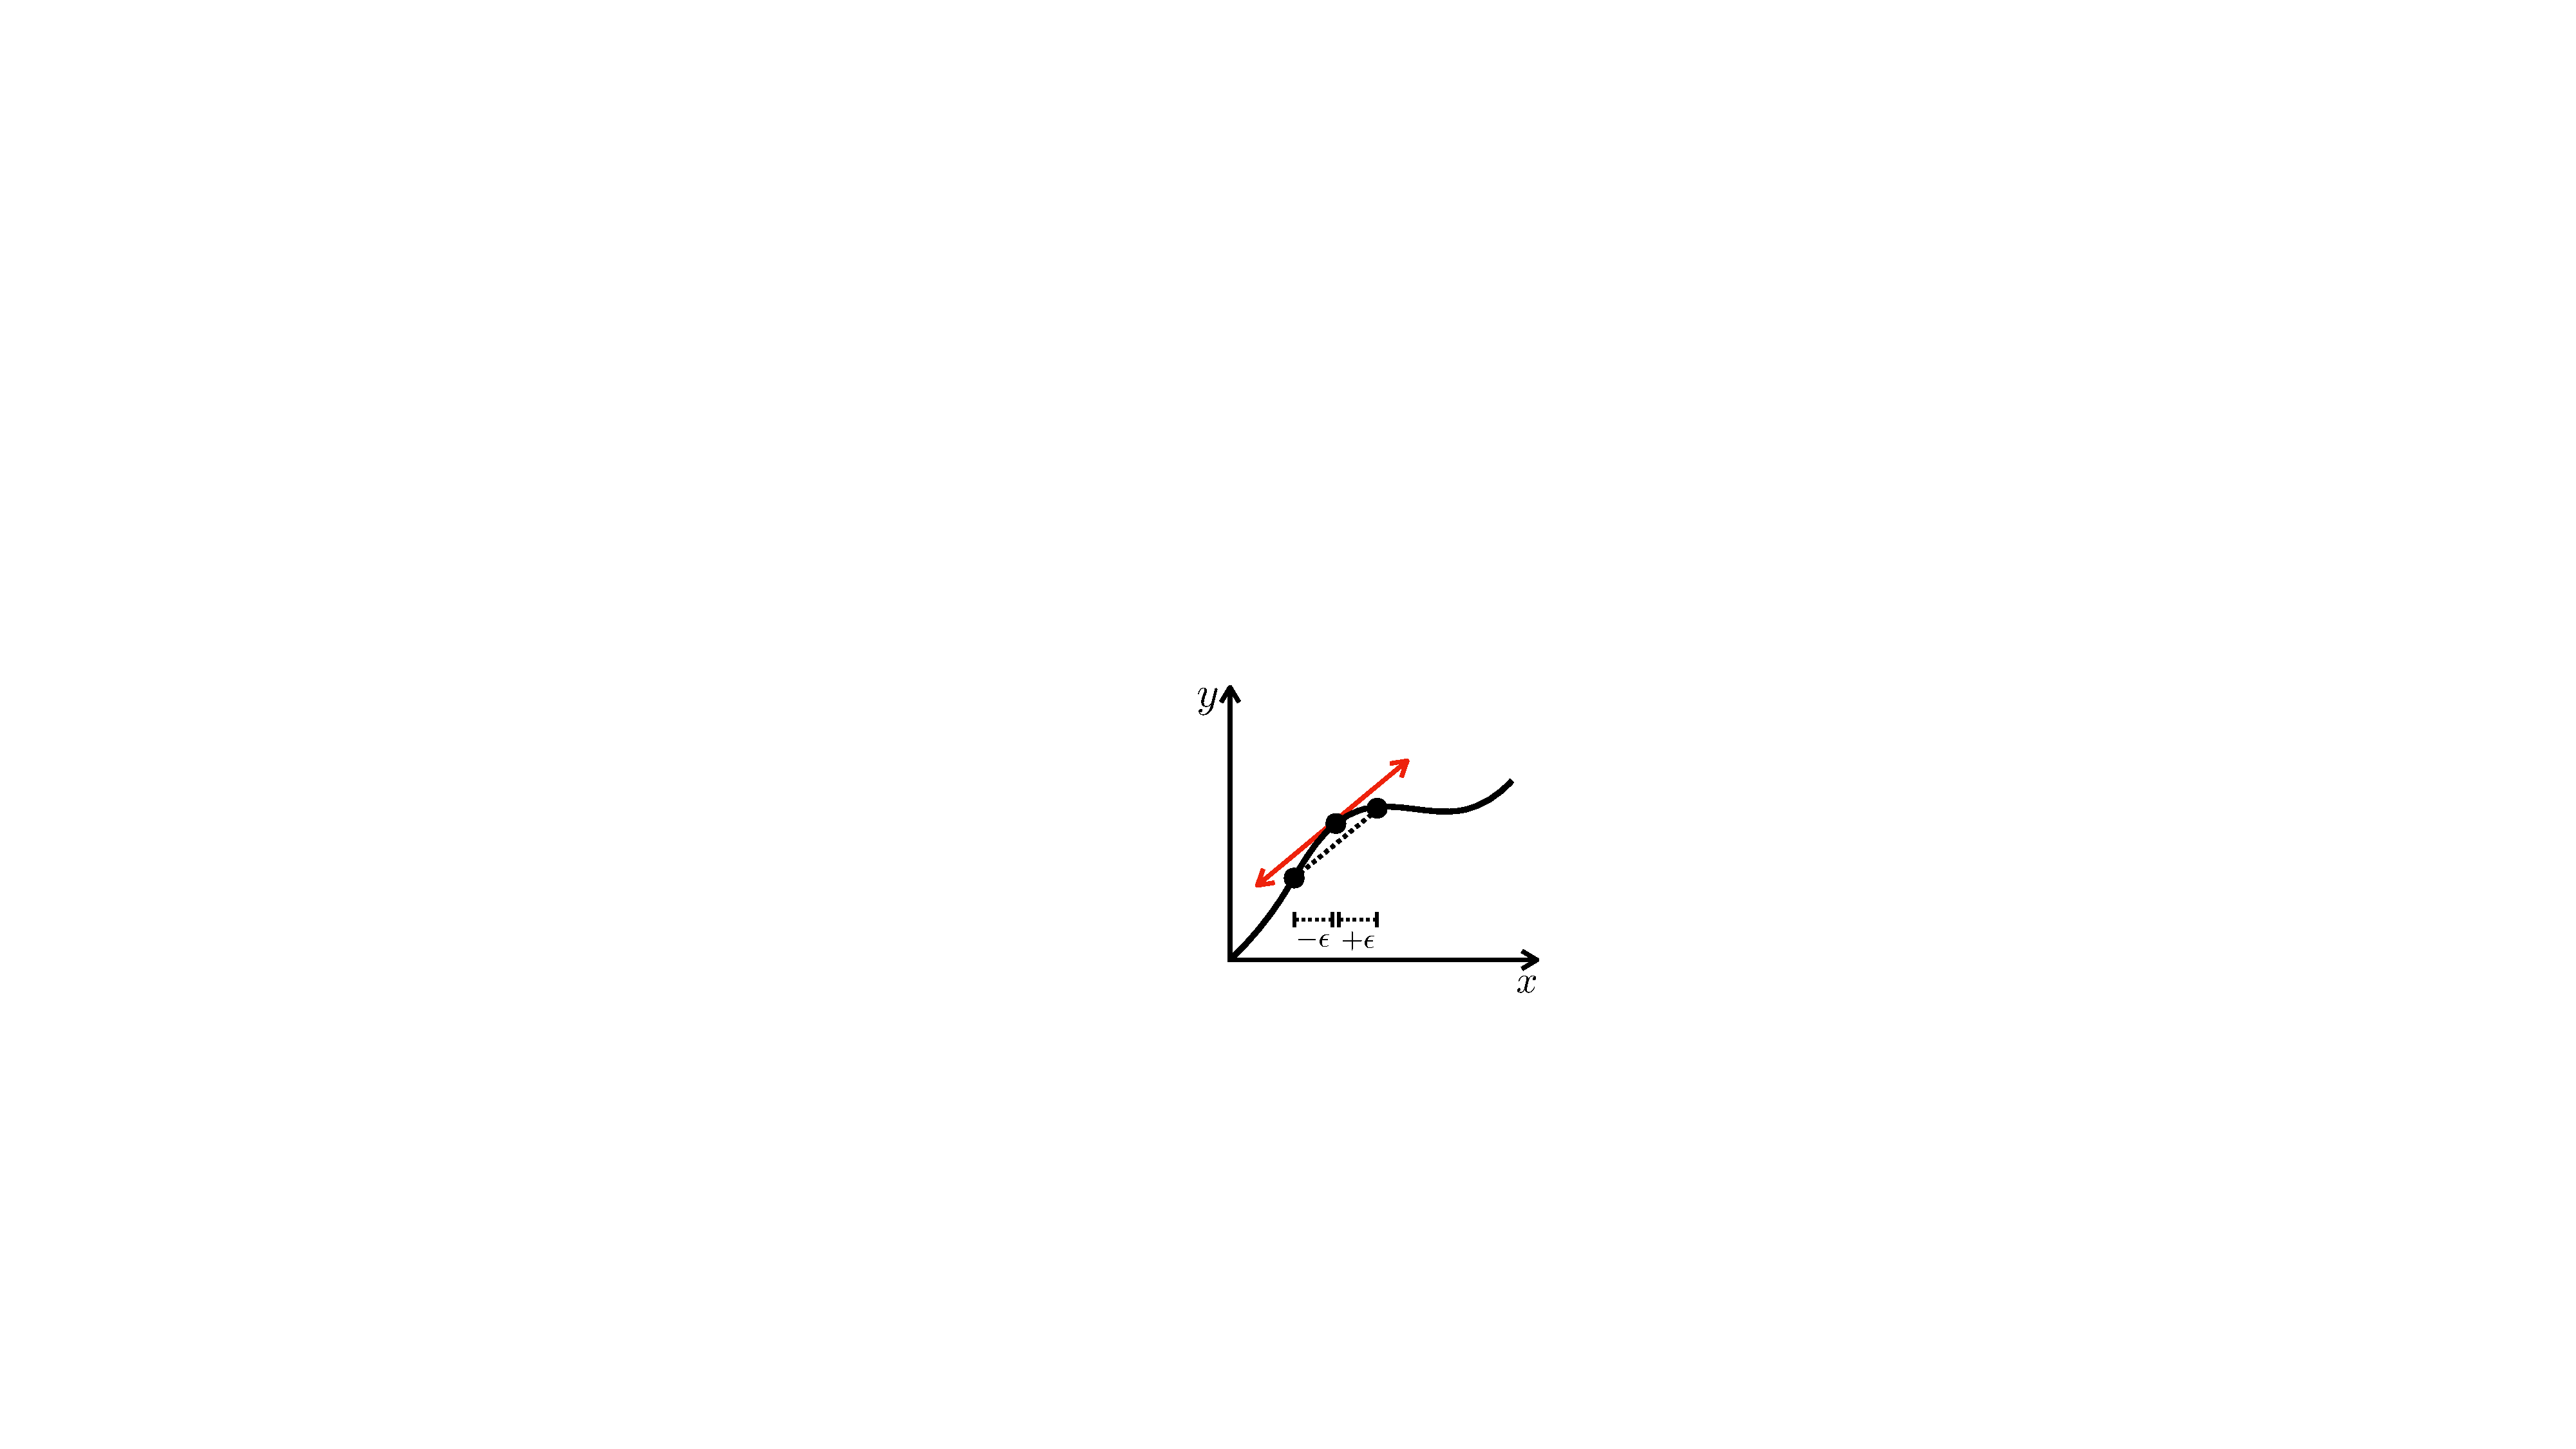
\includegraphics[width=0.35\linewidth]{./figures/gradient_descent/finite_diffs.pdf}
%     \label{fig-gradient_descent-finite_diffs}
% \end{figure}


%\section{Learning rate schedules}


\section{Stochastic Gradient Descent}\label{sec-gradient_descent-SGD}

One problem with the gradient-based methods we have seen so far is that the gradient may in fact be very expensive to compute, and this is often the case for learning problems. This is because learning problems typically have the form that $J$ is the average of losses incurred on each training datapoint. Computing $\nabla_{\theta}J(\theta)$ requires computing the gradient for each element in the average, that is, the gradient of the function being learned evaluated at the location of each datapoint in the training set. If we train on a big dataset, say 1 million training points, then to perform just \textit{one} step of gradient descent requires computing 1 million gradients! %. If we train on big data, which often we want to do, then even just evaluating $J$, or its gradient, will be expensive.
To make this clear, we will write out $J$ as an explicit function of the training data $\{\mathbf{x}^{(i)}, \mathbf{y}^{(i)}\}_{i=1}^N$. For typical learning problems, $\nabla_{\theta} J(\theta, \{\mathbf{x}^{(i)}, \mathbf{y}^{(i)}\}_{i=1}^N)$ decomposes as follows:
\begin{align}
    \nabla_{\theta} J(\theta, \{\mathbf{x}^{(i)}, \mathbf{y}^{(i)}\}_{i=1}^N) &= %\frac{1}{N}\sum_{i=1}^N \nabla_{\theta} \mathcal{J}(\theta, \mathbf{x}^{(i)}, \mathbf{y}^{(i)})\\
    %&= 
    \nabla_{\theta} \frac{1}{N}\sum_{i=1}^N \mathcal{L}(f_{\theta}(\mathbf{x}^{(i)}), \mathbf{y}^{(i)})\\
    &= \frac{1}{N}\sum_{i=1}^N \nabla_{\theta} \mathcal{L}(f_{\theta}(\mathbf{x}^{(i)}), \mathbf{y}^{(i)})
\end{align}

For large $N$, computing this sum is very expensive. Suppose instead we randomly subsample (without replacement) a \textit{batch} of terms from this sum, $\{\mathbf{x}^{(b)}, \mathbf{y}^{(b)}\}_{b=1}^B$, where $B$ is the \index{Batch size}\textbf{batch size}. We then compute an \textit{estimate} of the total gradient as the average gradient over this batch as follows:
\begin{align}
    \tilde{\mathbf{g}} = \frac{1}{N}\sum_{b=1}^B \nabla_{\theta} \mathcal{L}(f_{\theta}(\mathbf{x}^{(b)}), \mathbf{y}^{(b)})
\end{align}
If we sample a large batch, where $B$ is almost as large as $N$, then the average over the $B$ terms should be roughly the same as the average over all $N$ terms. If we sample a smaller batch, then our estimate of the gradient will be less accurate but faster to compute. Therefore we have a tradeoff between accuracy and speed, and we can navigate this tradeoff with the hyperparameter $B$. The variant of gradient descent that uses this idea is called \index{Stochastic gradient descent}\textbf{stochastic gradient descent} (SGD), because each iteration of descent uses a different randomly (stochastically) sampled batch of training data to estimate the gradient. The full description of \SGD~is given in \algref{\ref{alg-gradient_descent-SGD}}.
\begin{algorithm}[h]
\SetAlgoVlined
\DontPrintSemicolon
%\marginnote{{\bf Algorithm \ref{alg-gradient_descent-SGD}}: Stochastic gradient descent estimates the gradient from a stochastic subset (batch) of the full training data, and makes an update on that basis.}
\caption{{\bf Algorithm \ref{alg-gradient_descent-SGD}}: Stochastic gradient descent (\SGD). Stochastic gradient descent estimates the gradient from a stochastic subset (batch) of the full training data, and makes an update on that basis.}
\fakealgorithmcaption{}
\label{alg-gradient_descent-SGD}
{\bf Input:} initial parameter vector $\theta^{0}$, data $\{\mathbf{x}^{(i)},\mathbf{y}^{(i)}\}_{i=1}^N$, learning rate $\eta$, batch size $B$, number of steps $K$\;
{\bf Output:} trained parameter vector $\theta^* = \theta^K$\;
\For{\upshape $k= 0, \dots, K-1$}{
    $\{\mathbf{x}^{(b)},\mathbf{y}^{(b)}\}_{b=1}^B \sim \{\mathbf{x}^{(i)},\mathbf{y}^{(i)}\}_{i=1}^N \quad\quad \triangleleft \text{ sample batch of training data}$\;
    $\tilde{\mathbf{g}} = \frac{1}{N}\sum_{b=1}^B \nabla_{\theta} \mathcal{L}(f_{\theta}(\mathbf{x}^{(b)}), \mathbf{y}^{(b)})$\;
    $\theta^{k} \leftarrow \theta^{k-1} - \eta \tilde{\mathbf{g}}$\;
}
\end{algorithm}

\SGD~has a number of useful properties beyond just being faster to compute than \GD. Because each step of descent is somewhat random, \SGD~can jump over small bumps in the loss landscape, as long those bumps disappear for some randomly sampled batches. Another important property is that \SGD~can implicitly regularize the learning problem. For example, for linear problems (i.e., $f_\theta$ is linear), then if there are multiple parameter settings that minimize the loss, \SGD~will often converge to the solution with minimum parameter norm~\cite{zhang2021understanding}.

%\section{How to initialize?}

% \section{Parameterization matters}
% \reviewcomment{Unfinished section.}
% \subsection{The power of overparameterization}
% Show a problem where the overparameterized loss landscape has smooth paths of descent (around obstacles) but the less-parameterized loss landscape does not.

\section{Concluding Remarks}
The study of optimization can fill dozens of textbooks and thousands of academic papers. But fortunately for us, modern machine learning has converged on just a few very simple optimization methods that are used in practice. We will soon encounter deep learning, which is the main kind of machine learning used for computer vision. In deep learning, gradient-based optimization is the workhorse. Believe it or not, the handful of algorithms described above are enough to train most state-of-the-art deep learning models. Every year there are new elaborations on these ideas, and second-order methods are ever on the horizon, yet the basic concepts remain quite simple: compute a local estimate of the shape of the loss landscape, then, based on this shape, take a small step toward a lower loss.
%Sometimes this is even treated as definitional to deep learning: deep learning is learning with gradient-based optimization.